\documentclass{article}
\usepackage{amsmath,amssymb,graphicx,enumitem,wrapfig}

\begin{document}
\parindent=0cm
\parskip=6pt
\pagestyle{empty}

%Begin
%Language English
%Source Cariboo College High School Mathematics competition
%Title Senior Preliminary Round 1973
%Question 1
%Subject functions
%Category concepts
%Type MC
%Choices 5
%Answer B
%Creator Victor Semenoff
%Rdifficulty 18
%Qtext

\scriptsize
Source: Cariboo College High School Mathematics Contest

\normalsize
%\begin{wrapfigure}[2]{r}[0pt]{0pt}
%	\includegraphics[width=30mm,viewport=]{CCJ78-04}
%\end{wrapfigure}
If $2x+y=7$ and $y=4$, then $8x+y$ equals:\\
%ChoiceA
(A) -1\\
%ChoiceB
(B) 16\\
%ChoiceC
(C) 24\\
%ChoiceD
(D) 28\\
%ChoiceE
(E) 60\\
%Ftext

%\begin{wrapfigure}{r}[0pt]{0pt}
%	\includegraphics[width=30mm,viewport=]{CCJ78-04}
%\end{wrapfigure}

\textbf{The correct answer is (B): 16}\\[1 ex]
\begin{align*}
2x+y&=7\\
2x+4&=7\\
2x&=3\\
8x&=12\\
8x+y&=12+y=12+4=16.
\end{align*}
%End
\\[5 ex]
%Begin
%Language English
%Source Cariboo College High School Mathematics competition
%Title Senior Preliminary Round 1973
%Question 2
%Subject functions
%Category concepts
%Type MC
%Choices 5
%Answer E
%Creator Victor Semenoff
%Rdifficulty 15
%Qtext

\scriptsize
Source: Cariboo College High School Mathematics Contest

\normalsize
%\begin{wrapfigure}[2]{r}[0pt]{0pt}
%	\includegraphics[width=30mm]{CCJ78-04}
%\end{wrapfigure}
If $f(x)=10^x$ , then $f(x+1)-f(x)$ equals:\\
%ChoiceA
(A) 10\\
%ChoiceB
(B) 90\\
%ChoiceC
(C) $f(x)$\\
%ChoiceD
(D) $f(x)-1$\\
%ChoiceE
(E) $9f(x)$\\
%Ftext

%\begin{wrapfigure}{r}[0pt]{0pt}
%	\includegraphics[width=30mm]{CCJ78-04}
%\end{wrapfigure}

\textbf{The correct answer is (E): $9f(x)$}\\
\begin{align*}
f(x+1)-f(x)&=10^{x+1}-10^x\\
&=10^{x}\times10-10^x\\
&=(10-1)10^x\\
&=9\times10^x=9f(x)
\end{align*}
%End
\\[5 ex]
%Begin
%Language English
%Source Cariboo College High School Mathematics competition
%Title senior Preliminary Round 1973
%Question 3
%Subject arithmetic
%Category integers
%Type MC
%Choices 5
%Answer E
%Creator Victor Semenoff
%Rdifficulty 12
%Qtext

\scriptsize
Adapted From: Cariboo College High School Mathematics Contest

\normalsize
%\begin{wrapfigure}[2]{r}[0pt]{0pt}
%	\includegraphics[width=30mm]{CCJ78-04}
%\end{wrapfigure}
Which of the following  \textbf{is} divisible by 6?\\
%ChoiceA
(A) 4285\\
%ChoiceB
(B) 4653\\
%ChoiceC
(C) 3421\\
%ChoiceD
(D) 2727\\
%ChoiceE
(E) 2286\\
%Ftext

%\begin{wrapfigure}{r}[0pt]{0pt}
%	\includegraphics[width=30mm]{CCJ78-04}
%\end{wrapfigure}

\textbf{The correct answer is (E): 2286}\\
Since $6=2\times3$, a number that is divisible by 6 must be both divisible by 2, and divisible by 3.  Of the numbers listed, only 2286 is even and thus divisible by two. Further, the sum of the digits of 2286 is 18, and 18 is divisible by 3 thus 2286 is as well. Therefore, 2286 is divisible by 6.
%End
\\[5 ex]
%Begin
%Language English
%Source Cariboo College High School Mathematics competition
%Title Senior Preliminary Round 1973
%Question 4
%Subject functions
%Category rational
%Type MC
%Choices 5
%Answer E
%Creator Victor Semenoff
%Rdifficulty 13
%Qtext

\scriptsize
Source: Cariboo College High School Mathematics Contest

\normalsize
%\begin{wrapfigure}[2]{r}[0pt]{0pt}
%	\includegraphics[width=30mm]{CCJ78-04}
%\end{wrapfigure}
If $a\neq b$, then $\frac{a^{2}+a-b^{2}-b}{a-b}$ equals:\\
%ChoiceA
(A) $a^{2}-b^{2}$\\
%ChoiceB
(B) $2a-2b$\\
%ChoiceC
(C) $a+b$\\
%ChoiceD
(D) $a^{2}-b$\\
%ChoiceE
(E) None of the above\\
%Ftext

%\begin{wrapfigure}{r}[0pt]{0pt}
%	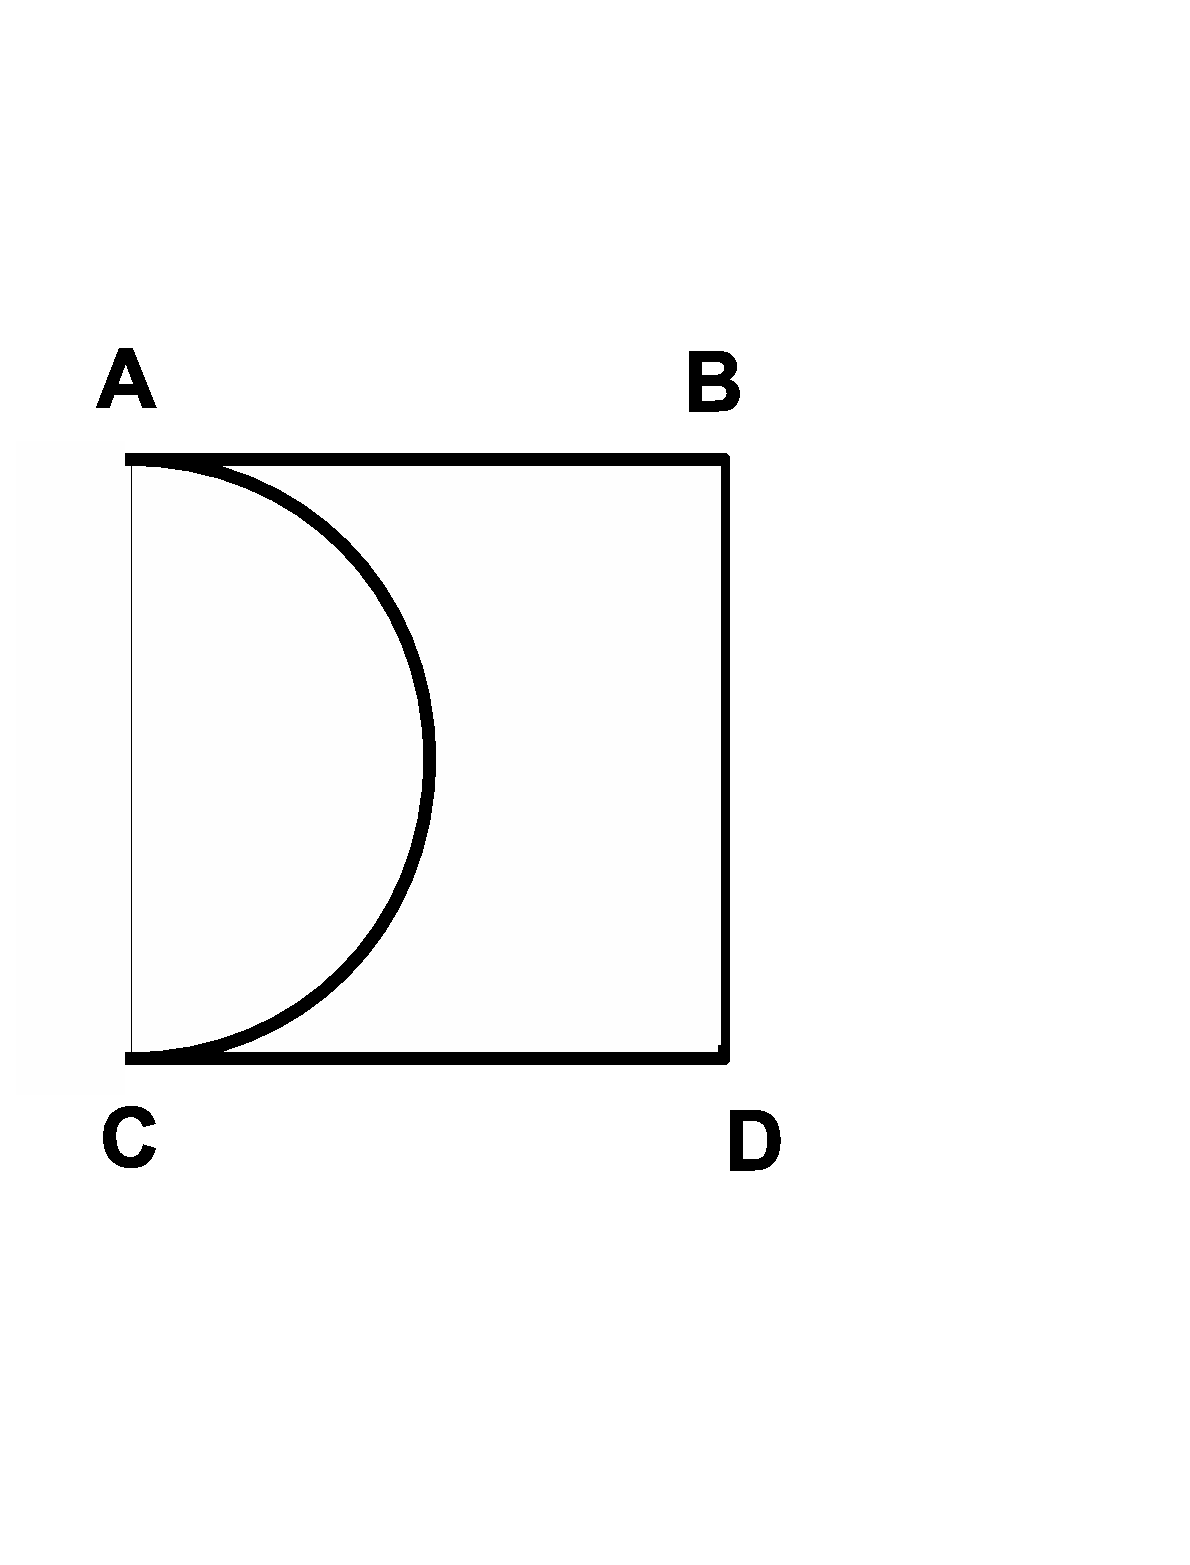
\includegraphics[width=30mm,viewport=22 224 351 579]{CCJPR74-4pic2.eps}
%\end{wrapfigure}

\textbf{The correct answer is (E): None of the above}\\
\begin{equation*}
\frac{a^{2}+a-b^{2}-b}{a-b}=\frac{a^{2}-b^{2}+a-b}{a-b}=\frac{(a+b)(a-b)+(a-b)}{a-b}=\frac{(a-b)(a+b+1)}{a-b}
\end{equation*}
Since $a\neq b$, we can cancel $(a-b)$ in the last line. Thus
\begin{equation*}
\frac{a^{2}+a-b^{2}-b}{a-b}=a+b+1.
\end{equation*}
%End
\\[5 ex]
%Begin
%Language English
%Source Cariboo College High School Mathematics competition
%Title Senior Preliminary Round 1973
%Question 5
%Subject arithmetic
%Category integers
%Type MC
%Choices 5
%Answer E
%Creator Victor Semenoff
%Rdifficulty 20
%Qtext

\scriptsize
Source: Cariboo College High School Mathematics Contest

\normalsize
%\begin{wrapfigure}[2]{r}[0pt]{0pt}
%	\includegraphics[width=30mm]{CCJ78-04}
%\end{wrapfigure}
If the integer $n$ is divided by 7, the remainder is 3.  What will be the remainder when $5n$ is divided by 7?\\
%ChoiceA
(A) 0\\
%ChoiceB
(B) 6\\
%ChoiceC
(C) 5\\
%ChoiceD
(D) 3\\
%ChoiceE
(E) 1\\
%Ftext

%\begin{wrapfigure}{r}[0pt]{0pt}
%	\includegraphics[width=30mm]{CCJ78-04}
%\end{wrapfigure}

\textbf{The correct answer is (E): 1}\\
Let $q$ be the quotient when $n$ is divided by 7. We can then write $n$ as $n=q+\frac{3}{7}$. Multiplying this equation by 5 gives:
\begin{equation*}
5n=5q+\frac{5\times3}{7}=5q+\frac{15}{7}= (5q+2)+\frac{1}{7}
\end{equation*}
From this we see that the remainder when $5n$ is divided by 7 is 1.
%End
\\[5 ex]
%Begin
%Language English
%Source Cariboo College High School Mathematics competition
%Title Senior Preliminary Round 1973
%Question 6
%Subject geometry
%Category triangles
%Type MC
%Choices 5
%Answer C
%Creator Victor Semenoff
%Rdifficulty 20
%Qtext

\scriptsize
Source: Cariboo College High School Mathematics Contest

\normalsize
\begin{wrapfigure}[4]{r}[0pt]{0pt}
	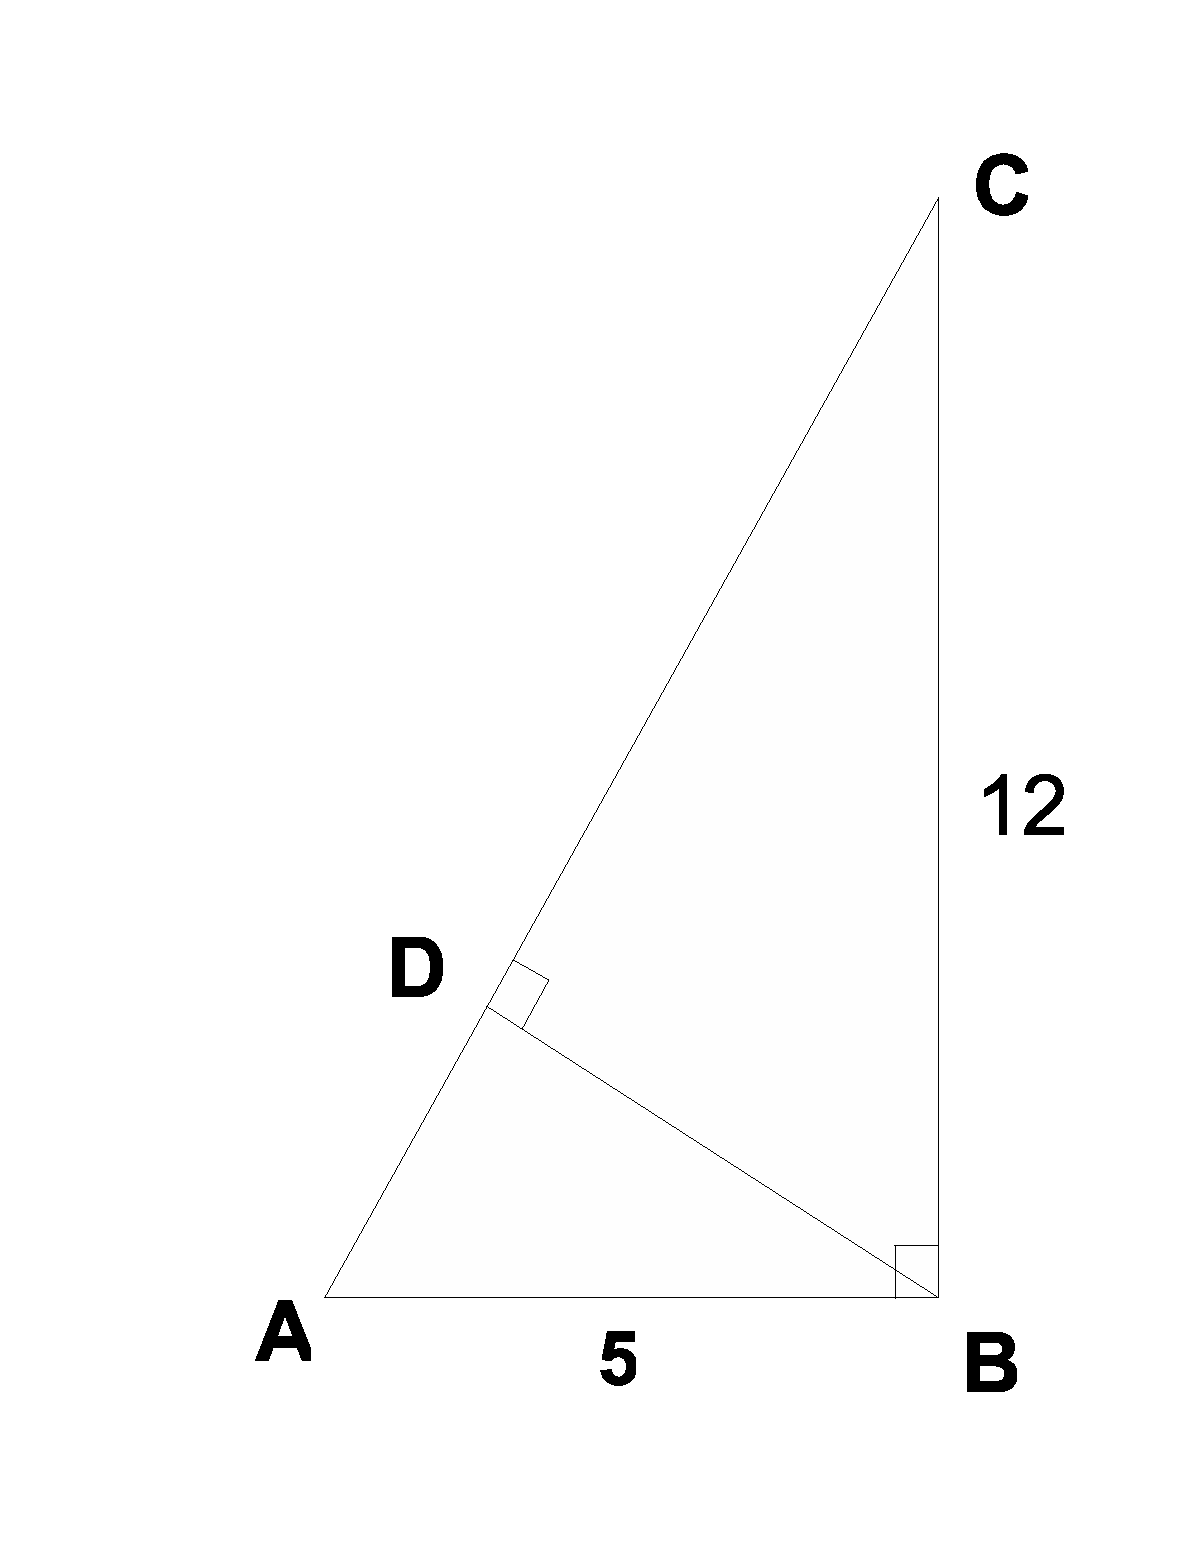
\includegraphics[width=25mm,viewport=100 67 508 675]{CCSPR73-6pic.eps}
\end{wrapfigure}
In triangle ABC, angle ABC is a right angle. If AB=5, BC=12, and angle BDC is a right angle, what is the length of BD?\\
%ChoiceA
(A) 5\\[1 ex]
%ChoiceB
(B) 13\\[1 ex]
%ChoiceC
(C) $\frac{60}{13}$\\[1 ex]
%ChoiceD
(D) $\frac{12}{13}$\\[1 ex]
%ChoiceE
(E) $\frac{17}{60}$\\
%Ftext

\begin{wrapfigure}{r}[0pt]{0pt}
	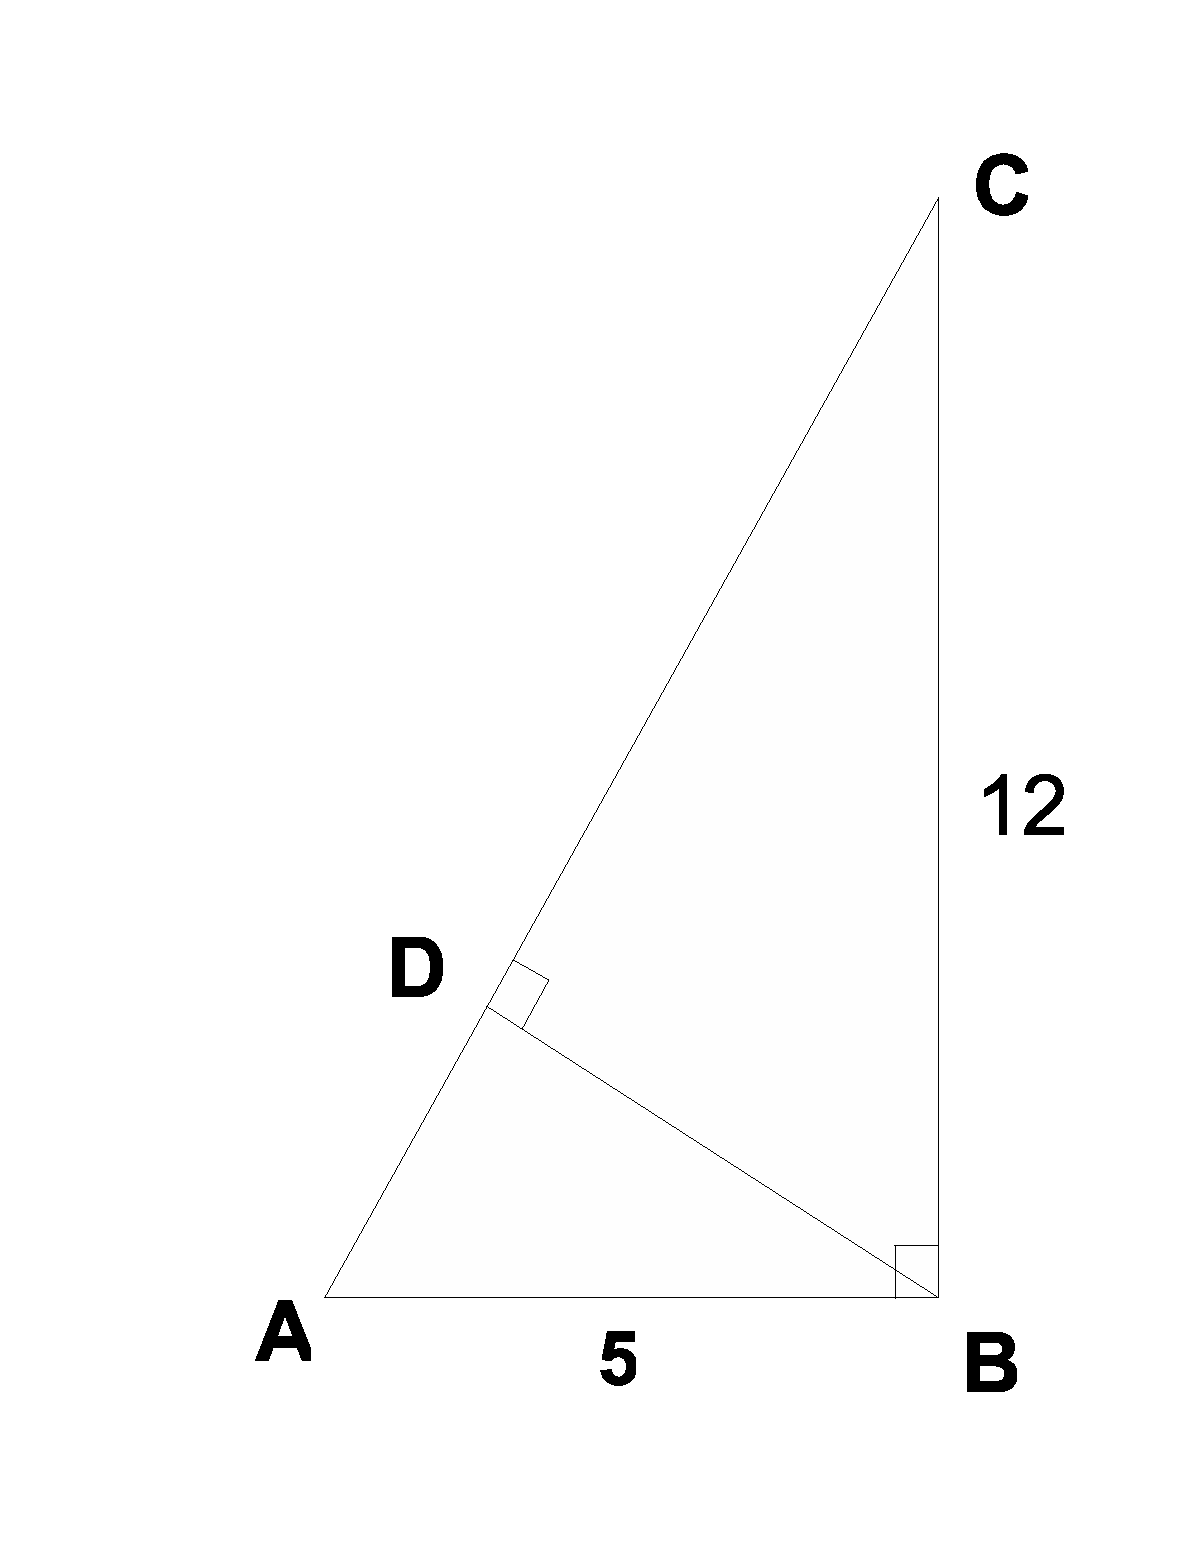
\includegraphics[width=25mm,viewport=100 67 508 675]{CCSPR73-6pic.eps}
\end{wrapfigure}
\textbf{The correct answer is (C): $\frac{60}{13}$}\\
Let A be the area of triangle ABC. Using AB as the base of the triangle, we find A$=\frac{1}{2}\times5\times12$. Since ABC is a right triangle, AC=13. If AC is then used as the base of ABC, and BD as its hight, we find A$=\frac{1}{2}\times13\times$BD. Thus
\begin{align*}
\frac{1}{2}\times5\times12&=\frac{1}{2}\times13\times\textrm{BD}\\
\textrm{BD}&=\frac{5\times12}{13}=\frac{60}{13}.
\end{align*}
%End
\\[5 ex]
%Begin
%Language English
%Source Cariboo College High School Mathematics competition
%Title Senior Preliminary Round 1973
%Question 7
%Subject geometry
%Category triangles
%Type MC
%Choices 5
%Answer A
%Creator Victor Semenoff
%Rdifficulty 25
%Qtext

\scriptsize
Source: Cariboo College High School Mathematics Contest

\normalsize
%\begin{wrapfigure}[2]{r}[0pt]{0pt}
%	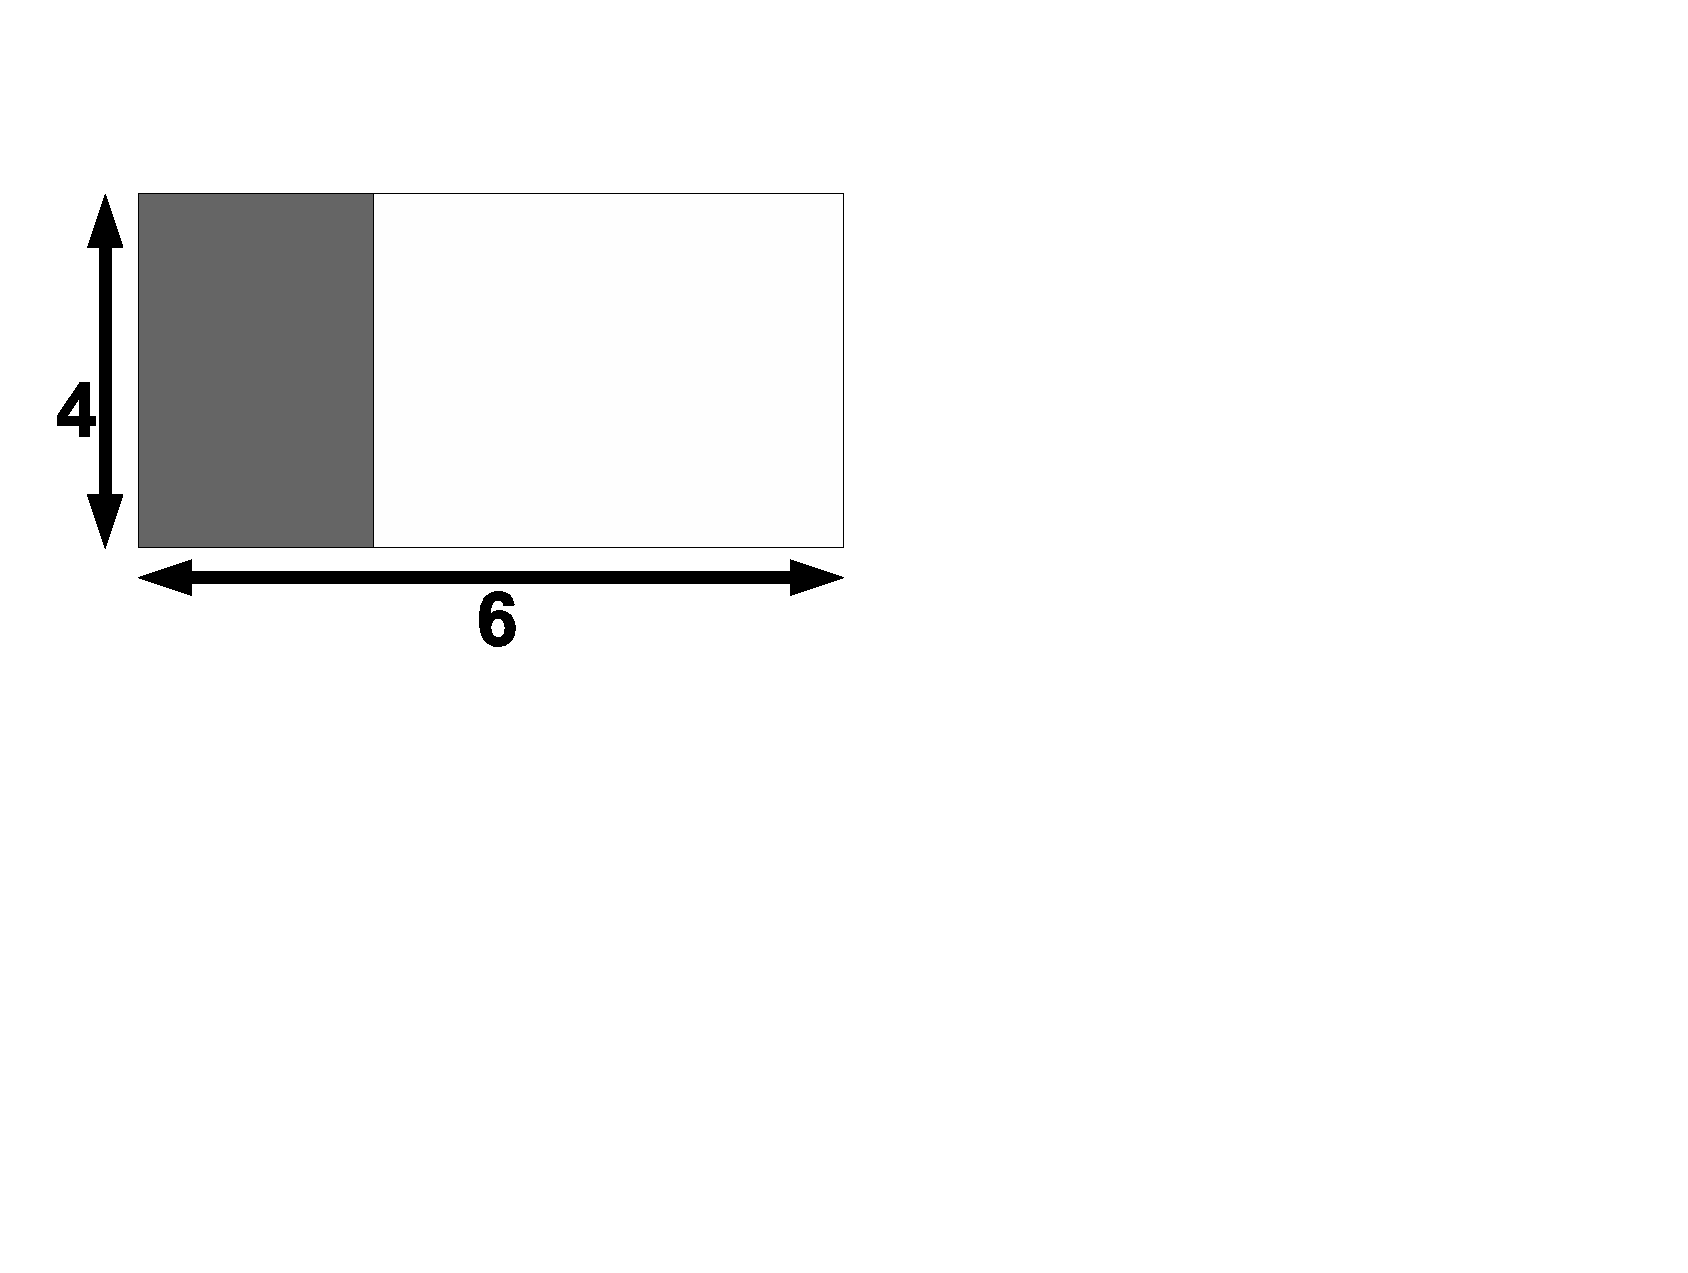
\includegraphics[width=30mm,viewport=17 290 402 516]{CCJPR73-7pic.eps}
%\end{wrapfigure}
If triangles A and B are similar and a side of A is 12 times the length of the corresponding side of B, how many times larger is the area of A than the area of B?\\
%ChoiceA
(A) 144\\
%ChoiceB
(B) 72\\
%ChoiceC
(C) 36\\
%ChoiceD
(D) 4\\
%ChoiceE
(E) Not enough information\\
%Ftext

%\begin{wrapfigure}{r}[0pt]{0pt}
%	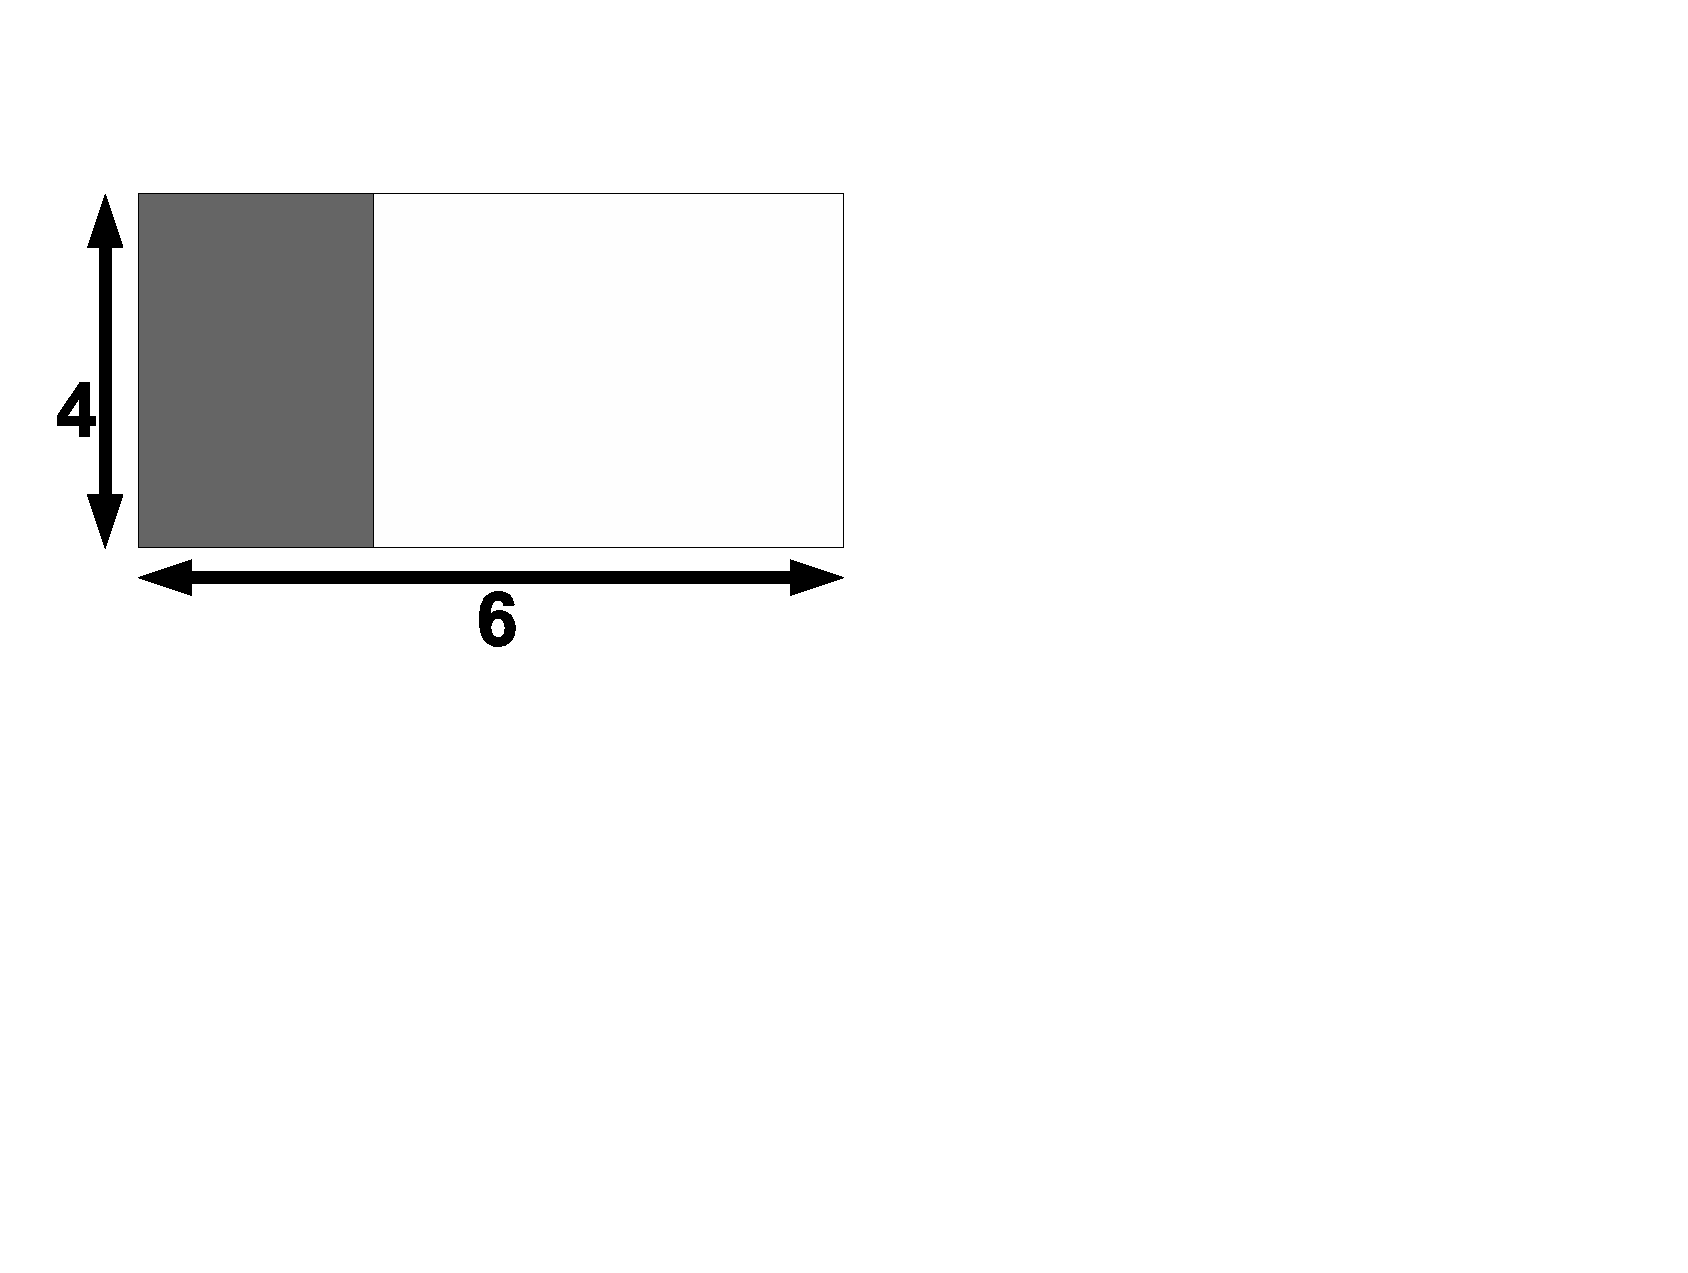
\includegraphics[width=30mm,viewport=17 290 402 516]{CCJPR73-7pic.eps}
%\end{wrapfigure}

\textbf{The correct answer is (A): 144}\\[1ex]
Imagine the altitudes and bases of triangles A and B drawn in similar manners. Since the triangles are similar, and one side of A is 12 times as long as the corresponding side of B, the altitude drawn on A would be 12 times the altitude drawn on B, while the base drawn on A would be 12 times the base drawn on B. Since the area of a triangle is proportional to the product of its base and its altitude, the area of triangle A would then be $12^{2}=144$ times the area of triangle B.
%End
\\[5 ex]
%Begin
%Language English
%Source Cariboo College High School Mathematics competition
%Title Senior Preliminary Round 1973
%Question 8
%Subject functions
%Category concepts
%Type MC
%Choices 5
%Answer B
%Creator Victor Semenoff
%Rdifficulty 18
%Qtext

\scriptsize
Source: Cariboo College High School Mathematics Contest

\normalsize
%\begin{wrapfigure}[2]{r}[0pt]{0pt}
%	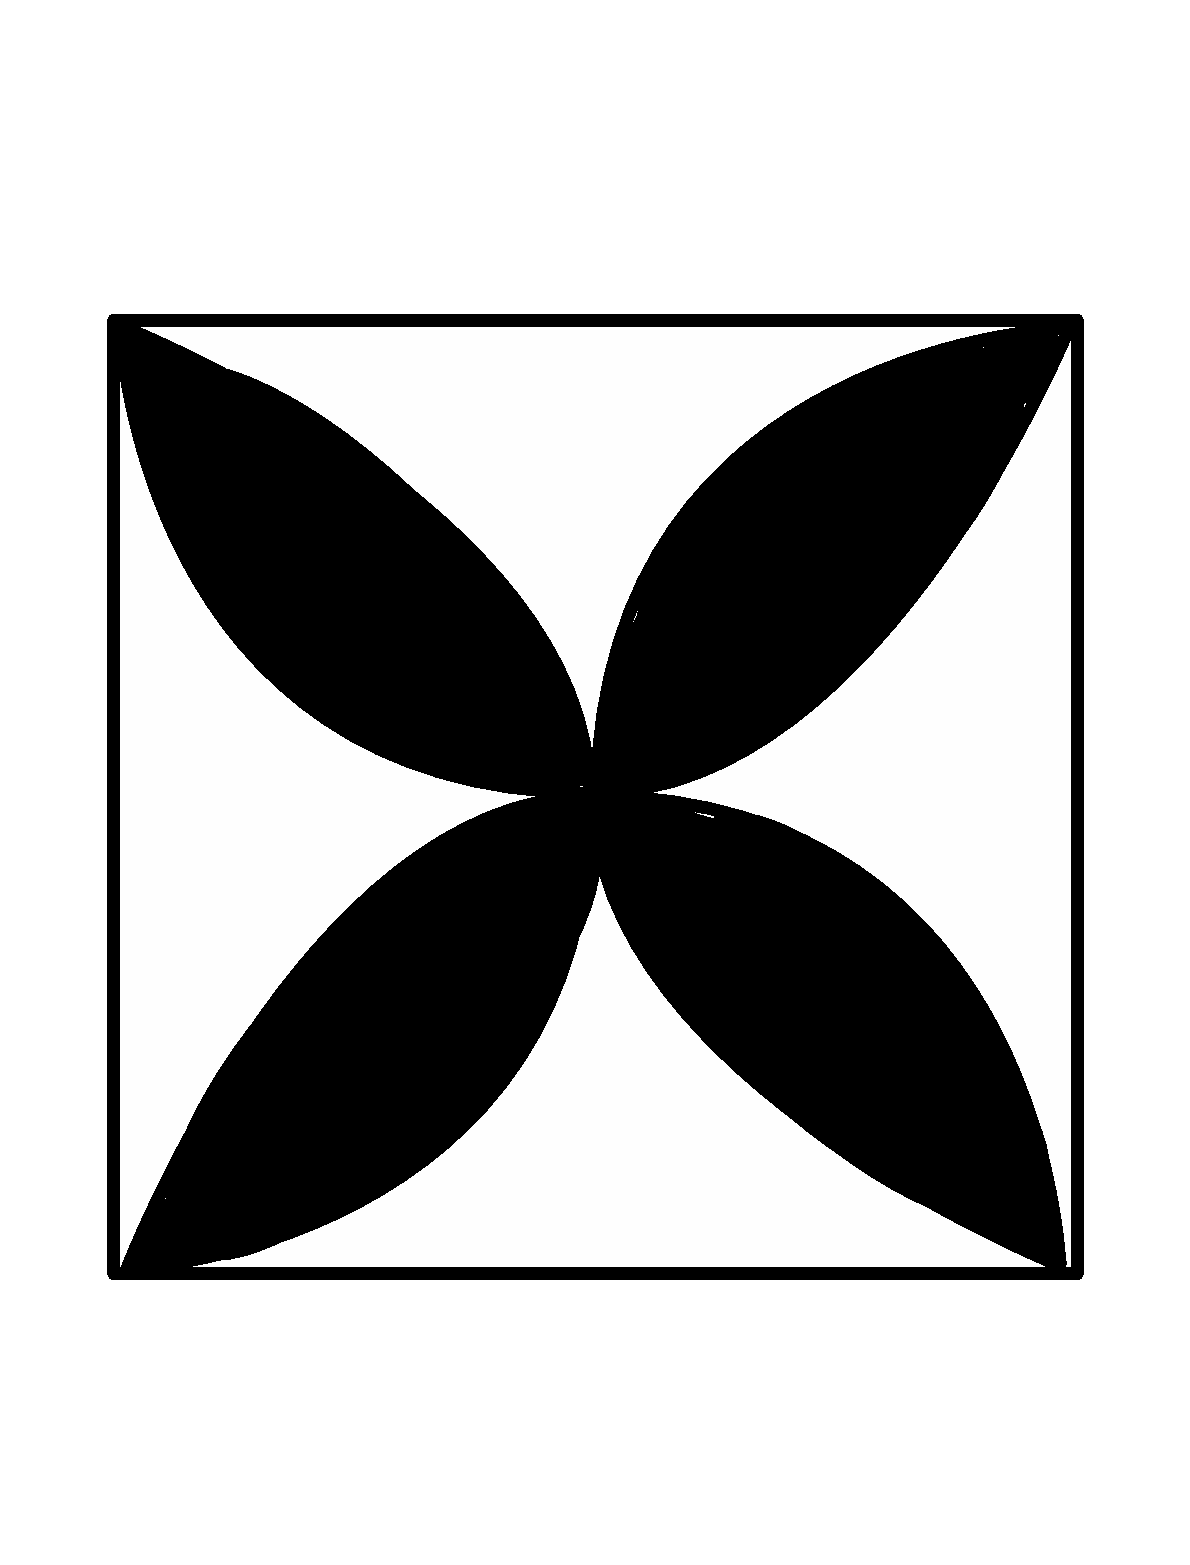
\includegraphics[width=30mm,viewport=36 122 514 596]{CCJPR74-8pic.eps}
%\end{wrapfigure}
If $f(x)=x+1$ and $F(x,y)=y^{2}+x$, then $F(2,f(3))$ equals:\\
%ChoiceA
(A) $x^{2}+3x+1$\\
%ChoiceB
(B) 18\\
%ChoiceC
(C) 8\\
%ChoiceD
(D) 4\\
%ChoiceE
(E) 1\\
%Ftext

%\begin{wrapfigure}{r}[0pt]{0pt}
%	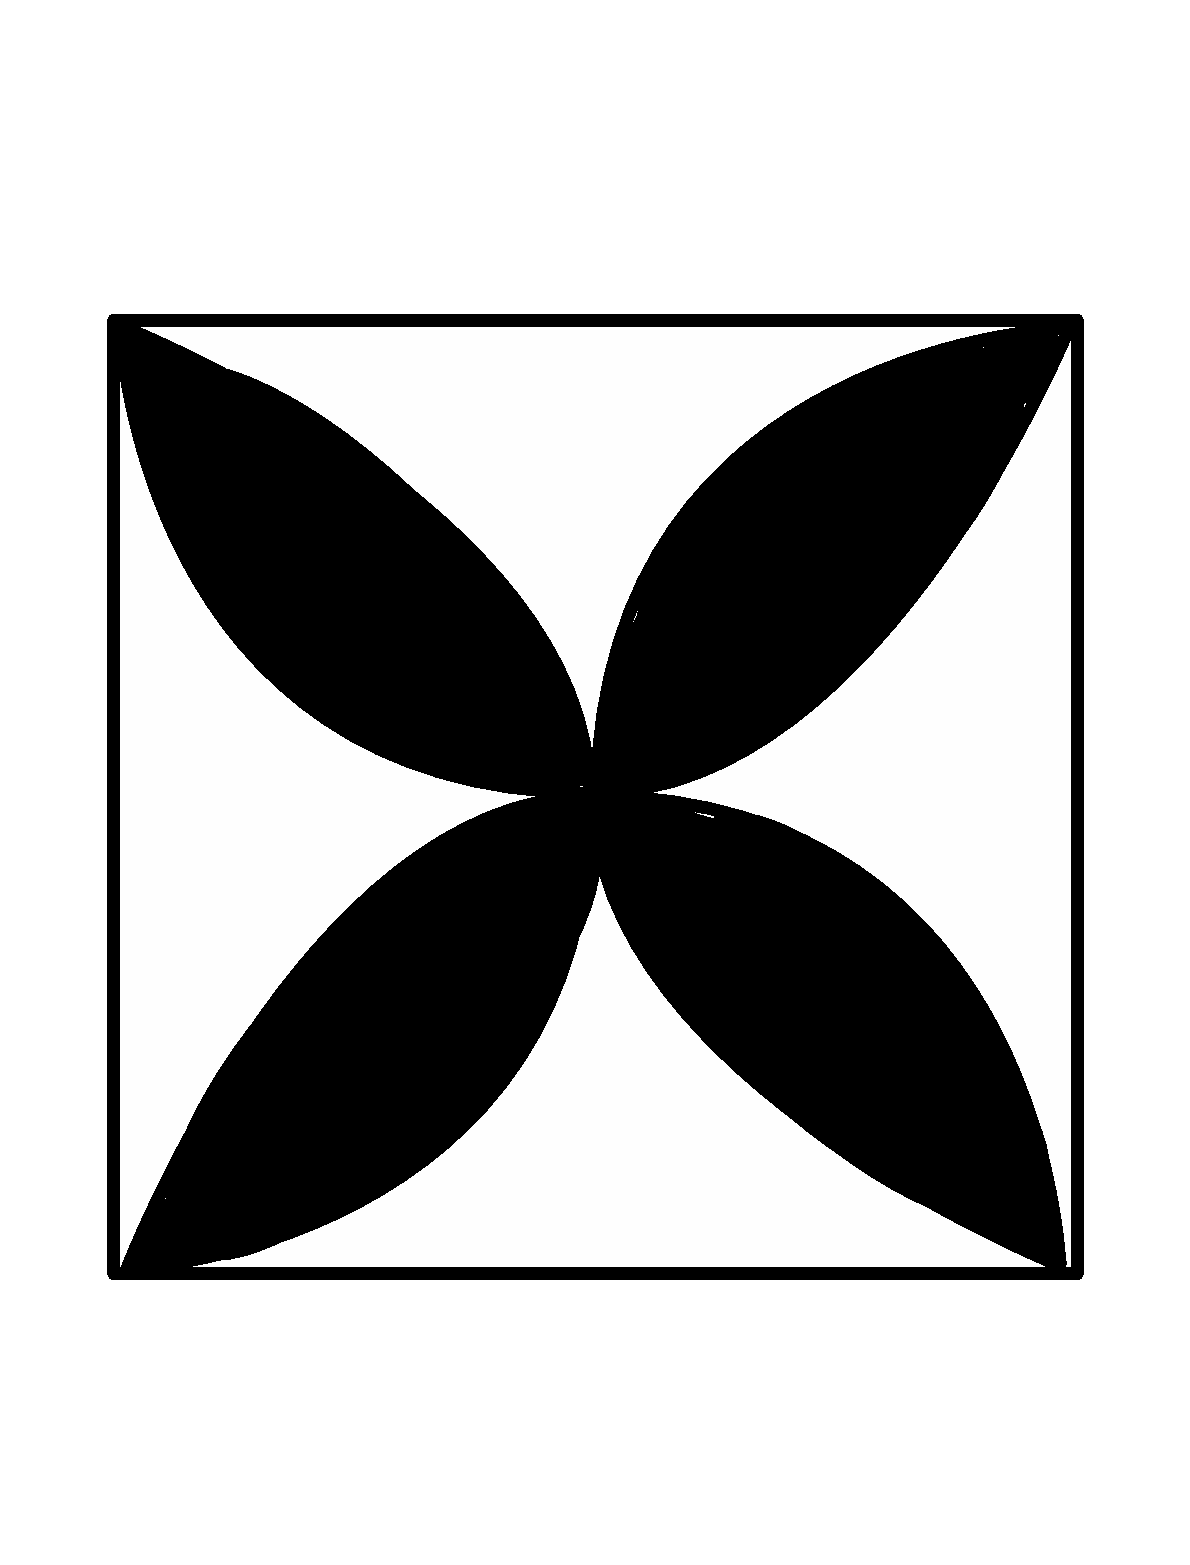
\includegraphics[width=30mm,viewport=36 122 514 596]{CCJPR74-8pic.eps}
%\end{wrapfigure}

\textbf{The correct answer is (B): 18}\\[1 ex]
\begin{equation*} 
F(2,f(3))=(f(3))^{2}+2=(3+1)^{2}+2=16+2=18
\end{equation*}
%End
\\[5 ex]
%Begin
%Language English
%Source Cariboo College High School Mathematics competition
%Title Senior Preliminary Round 1973
%Question 9
%Subject algebra
%Category modelling
%Type MC
%Choices 5
%Answer D
%Creator Victor Semenoff
%Rdifficulty 15
%Qtext

\scriptsize
Source: Cariboo College High School Mathematics Contest

\normalsize
%\begin{wrapfigure}[2]{r}[0pt]{0pt}
%	\includegraphics[width=30mm,viewport=]{CCJ78-04}
%\end{wrapfigure}
In a certain chess tournament a player is eliminated if he loses a game. If there were 40 contestants and no game ended in a draw, the number of games played to determine the final winner was:\\
%ChoiceA
(A) 160\\
%ChoiceB
(B) 80\\
%ChoiceC
(C) 40\\
%ChoiceD
(D) 39\\
%ChoiceE
(E) 20\\
%Ftext

%\begin{wrapfigure}{r}[0pt]{0pt}
%	\includegraphics[width=30mm,viewport=]{CCJ78-04}
%\end{wrapfigure}

\textbf{The correct answer is (D): 39}\\[1 ex]
Each game played eliminates one player, and as we must eliminate 39 to determine a winner, 39 games must be played.
%End
\\[5 ex]
%Begin
%Language English
%Source Cariboo College High School Mathematics competition
%Title Senior Preliminary Round 1973
%Question 10
%Subject geometry
%Category area
%Type MC
%Choices 5
%Answer A
%Creator Victor Semenoff
%Rdifficulty 25
%Qtext

\scriptsize
Source: Cariboo College High School Mathematics Contest

\normalsize
\begin{wrapfigure}[4]{r}[0pt]{0pt}
	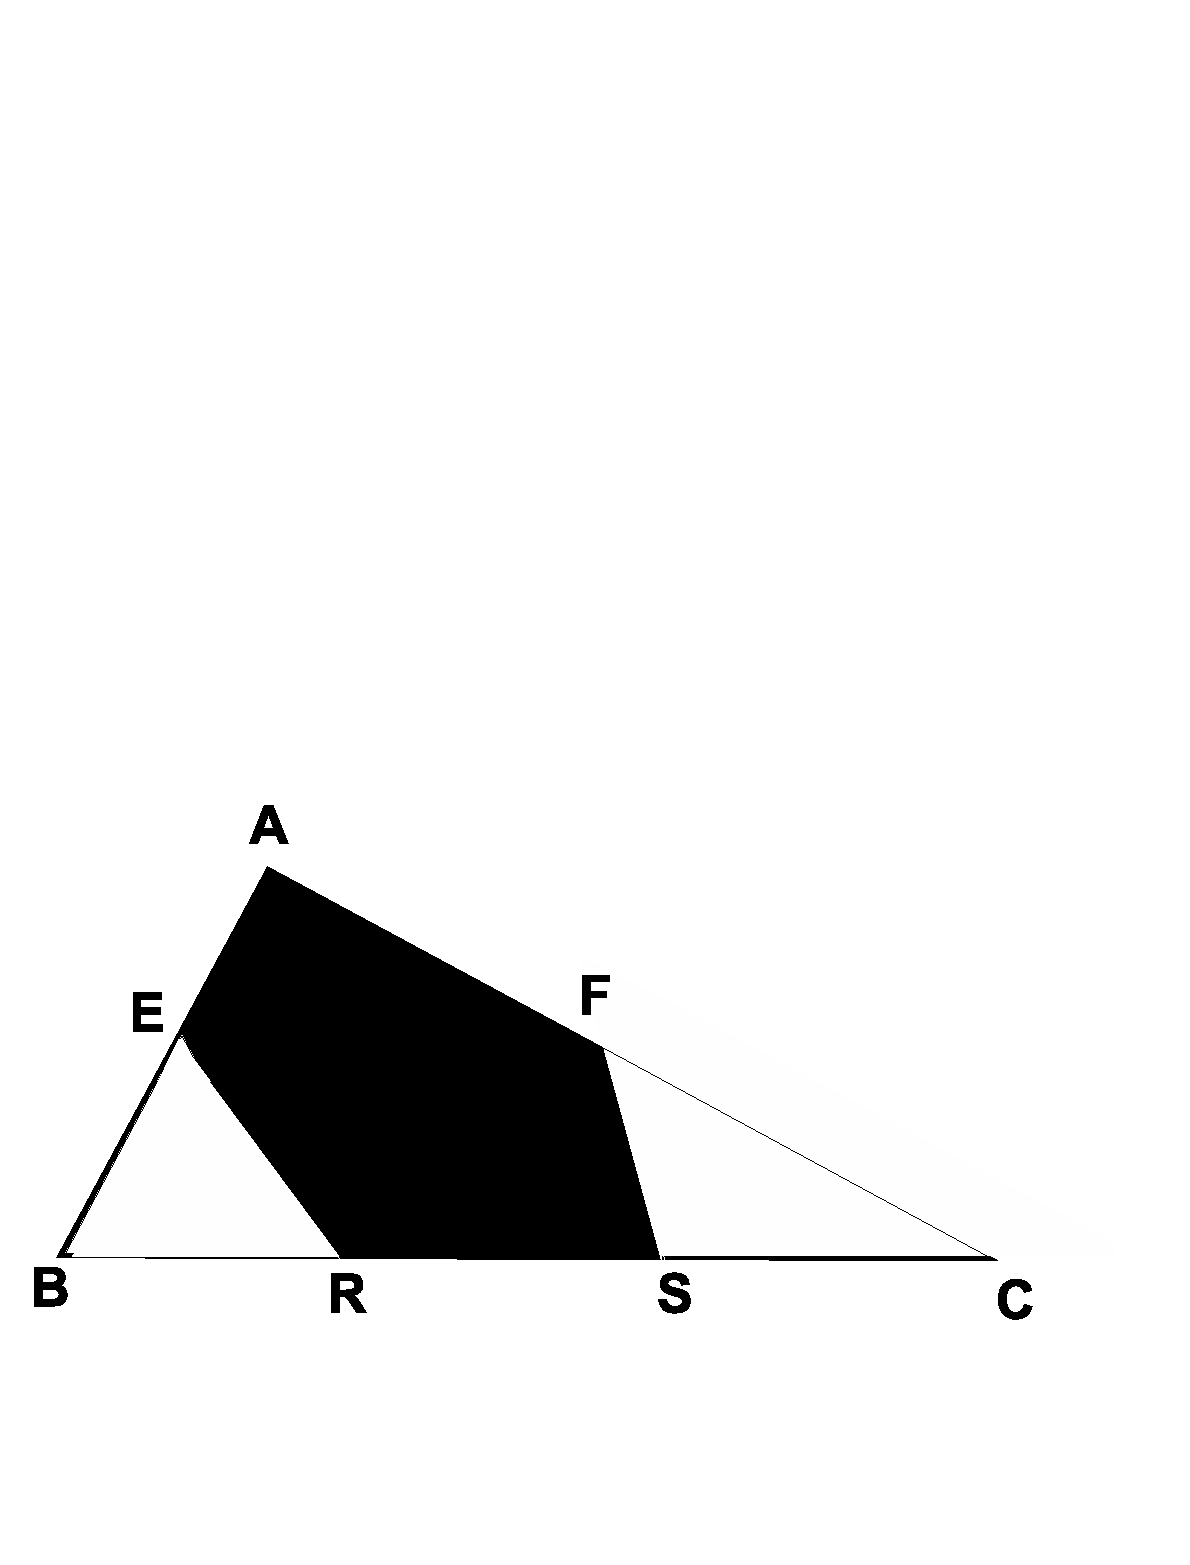
\includegraphics[width=35mm,viewport=4 102 497 362]{CCSPR73-10pic.eps}
\end{wrapfigure}
In the figure, E is the mid-point of AB, F is the mid-point of AC, and BR=RS=SC. If the area of triangle ABC is 252, what is the area of the shaded region?\\
%ChoiceA
(A) 168\\
%ChoiceB
(B) 189\\
%ChoiceC
(C) 201$\frac{3}{5}$\\
%ChoiceD
(D) 210\\
%ChoiceE
(E) 220\\
%Ftext\\

\begin{wrapfigure}{r}[0pt]{0pt}
	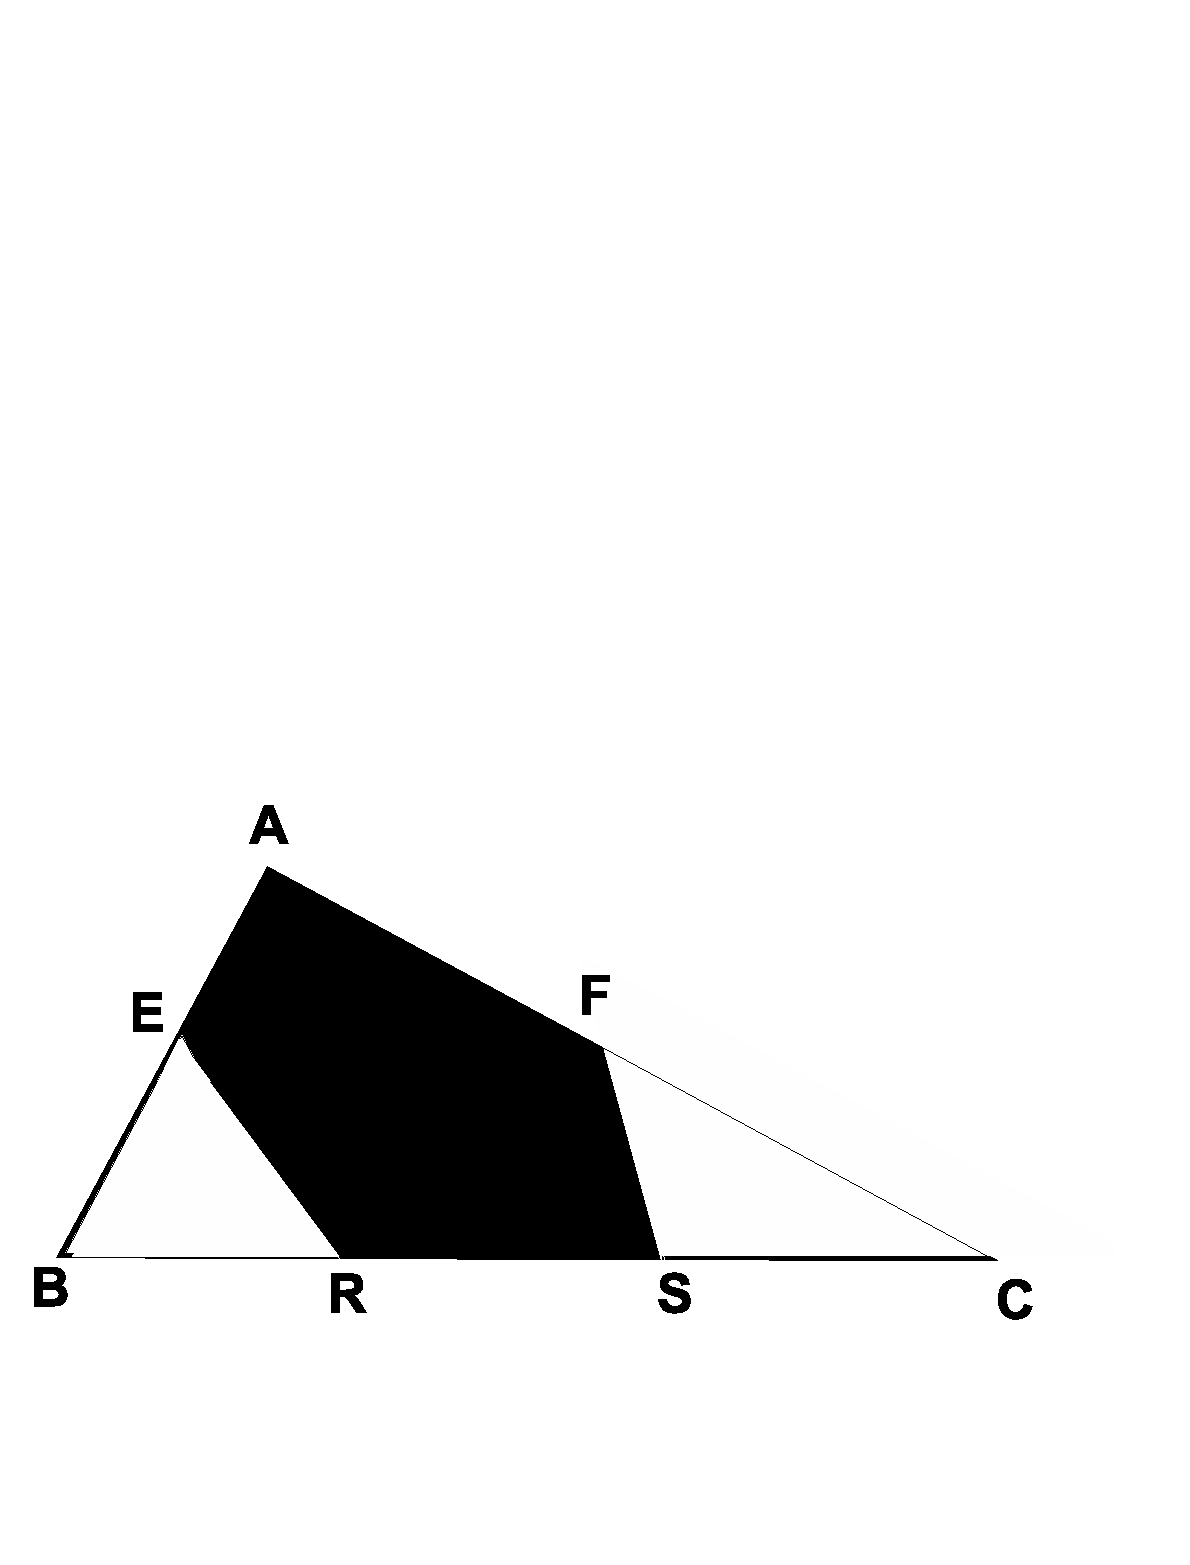
\includegraphics[width=35mm,viewport=4 102 497 362]{CCSPR73-10pic.eps}
\end{wrapfigure}

\textbf{The correct answer is (A): 168}\\[1 ex]
Since EB is half the length of AB, the area of triangle EBC is one half that of ABC, ie., 126.  (We can argue this by considering AB and EB as the bases of the triangles.) A similar argument shows that triangle FCB also has half the area of triangle ABC, ie. 126. Since BR is one third the length of BC, we can argue that the area of triangle EBR is one third that of triangle EBC, ie., triangle EBR has area 42. Similarly, triangle FCS has one third the area of FCB, ie., it also has area 42. Thus the area of the shaded region is $252-42-42=168$.
%End
\\[5 ex]
%Begin
%Language English
%Source Cariboo College High School Mathematics competition
%Title Senior Preliminary Round 1973
%Question 11
%Subject geometry
%Category length
%Type MC
%Choices 5
%Answer D
%Creator Victor Semenoff
%Rdifficulty 23
%Qtext

\scriptsize
Source: Cariboo College High School Mathematics Contest

\normalsize
%\begin{wrapfigure}[2]{r}[0pt]{0pt}
%	\includegraphics[width=30mm,viewport=]{CCJ78-04}
%\end{wrapfigure}
A 24 foot ladder leans against a wall so that the bottom of the ladder is 8 feet from the wall. How far from the wall (in inches) is the ladder at the point 4 feet from the top of the ladder?\\
%ChoiceA
(A) 80\\
%ChoiceB
(B) 24\\
%ChoiceC
(C) 20\\
%ChoiceD
(D) 16\\
%ChoiceE
(E) 12\\
%Ftext

%\begin{wrapfigure}{r}[0pt]{0pt}
%	\includegraphics[width=30mm,viewport=]{CCJ78-04}
%\end{wrapfigure}

\textbf{The correct answer is (D): 16}\\[1 ex]
Let $x$ be the distance we are looking for (in feet). When we sketch the situation, we obtain two similar, right triangles: one with a side of length 8 and hypotenuse of length 24, and one with a side of length $x$ and hypotenuse of length 4. By the law of similar triangles:
\begin{align*}
\frac{x}{4}&=\frac{8}{24}\\
x&=\frac{8}{6}
\end{align*}
Since there are 12 inches in a foot, we see that $x=12\times\frac{8}{6}=16$ inches.
%End
\\[5 ex]
%Begin
%Language English
%Source Cariboo College High School Mathematics competition
%Title Senior Preliminary Round 1973
%Question 12
%Subject algebra
%Category modelling
%Type MC
%Choices 5
%Answer C
%Creator Victor Semenoff
%Rdifficulty 24
%Qtext

\scriptsize
Source: Cariboo College High School Mathematics Contest

\normalsize
%\begin{wrapfigure}[2]{r}[0pt]{0pt}
%	\includegraphics[width=30mm,viewport=]{CCJ78-04}
%\end{wrapfigure}
Bill and Chuck are cycling from Kamloops towards Clearwater. They start at the same time.  Bill rides at 10 km/h and Chuck rides at 6 km/h. After Bill has been riding for 4 hours he turns back to Kamloops. How many kilometers has Chuck traveled when he meets Bill?\\
%ChoiceA
(A) 20\\
%ChoiceB
(B) 24\\
%ChoiceC
(C) 30\\
%ChoiceD
(D) 32\\
%ChoiceE
(E) 34\\
%Ftext

%\begin{wrapfigure}{r}[0pt]{0pt}
%	\includegraphics[width=30mm,viewport=]{CCJ78-04}
%\end{wrapfigure}

\textbf{The correct answer is (C): 30}\\[1 ex]
Bill will have traveled 10 km/h$\times4$h=40km before he turns back. In this same time Chuck will have traveled 6km/h$\times$4h=24km. Thus they will be 16 km apart when Bill turns around. They will now approach each other at the rate of 10km/h$+$6km/h=16km/h. Thus they will meet each other $\frac{16\textrm{km}}{16\textrm{km/h}}=1\textrm{h}$ after bill turned around. In this 1h Chuck will have traveled another 6km, making the total distance he travels 24km$+$6km=30km.
%End
\\[5 ex]
%Begin
%Language English
%Source Cariboo College High School Mathematics competition
%Title Senior Preliminary Round 1973
%Question 13
%Subject functions
%Category absval
%Type MC
%Choices 5
%Answer A
%Creator Victor Semenoff
%Rdifficulty 21
%Qtext

\scriptsize
Source: Cariboo College High School Mathematics Contest

\normalsize
%\begin{wrapfigure}[2]{r}[0pt]{0pt}
%	\includegraphics[width=30mm,viewport=]{CCJ78-04}
%\end{wrapfigure}
Given that $a<b$, $a>0$, and $b>0$ it is always true that:\\
%ChoiceA
(A) $\log{\frac{b}{a}}>0$\\[1 ex]
%ChoiceB
(B) $\log{\frac{a}{b}}>0$\\[1 ex]
%ChoiceC
(C) $\log{(b-a)}>0$\\[1 ex]
%ChoiceD
(D) $\log{a^b}>0$\\[1 ex]
%ChoiceE
(E) $\frac{\log{b}}{\log{a}}>0$\\
%Ftext

%\begin{wrapfigure}{r}[0pt]{0pt}
%	\includegraphics[width=30mm,viewport=]{CCJ78-04}
%\end{wrapfigure}

\textbf{The correct answer is (A): $\log{\frac{b}{a}}>0$}\\[1 ex]
Since $a>0$, dividing both sides of $a<b$ by $a$ leaves $1<\frac{b}{a}$ which is the same as $\frac{b}{a}>1$. Taking logarithms of both sides gives $\log{\frac{b}{a}}>0$. Counterexamples can easily be found for all the other answers.
%End
\\[5 ex]
%Begin
%Language English
%Source Cariboo College High School Mathematics competition
%Title Senior Preliminary Round 1973
%Question 14
%Subject geometry
%Category area
%Type MC
%Choices 5
%Answer D
%Creator Victor Semenoff
%Rdifficulty 16
%Qtext

\scriptsize
Source: Cariboo College High School Mathematics Contest

\normalsize
%\begin{wrapfigure}[2]{r}[0pt]{0pt}
%	\includegraphics[width=30mm,viewport=]{CCJ78-04}
%\end{wrapfigure}
The area of the triangle formed by the $x$-axis, the $y$-axis, and the line $2y+3x=12$ is:\\
%ChoiceA
(A) 24\\
%ChoiceB
(B) 36\\
%ChoiceC
(C) 18\\
%ChoiceD
(D) 12\\
%ChoiceE
(E) 6\\
%Ftext

%\begin{wrapfigure}{r}[0pt]{0pt}
%	\includegraphics[width=30mm,viewport=]{CCJ78-04}
%\end{wrapfigure}

\textbf{The correct answer is (D): 12}\\[1 ex]
The line crosses the $x$-axis at (4,0), and crosses the $y$-axis at (0,6). Thus the base of the triangle is 4, and its altitude is 6, for a total area of $\frac{1}{2}\times4\times6$=12.
%End
\\[5 ex]
%Begin
%Language English
%Source Cariboo College High School Mathematics competition
%Title Senior Preliminary Round 1973
%Question 15
%Subject geometry
%Category 3D
%Type MC
%Choices 5
%Answer D
%Creator Victor Semenoff
%Rdifficulty 19
%Qtext

\scriptsize
Source: Cariboo College High School Mathematics Contest

\normalsize
%\begin{wrapfigure}[2]{r}[0pt]{0pt}
%	\includegraphics[width=30mm,viewport=]{CCJ78-04}
%\end{wrapfigure}
The ratio of the total volume of three spheres each of radius 2 to the volume of a single sphere of radius 6 is:\\
%ChoiceA
(A) $1:1$\\
%ChoiceB
(B) $2:3$\\
%ChoiceC
(C) $4\pi:36\pi$\\
%ChoiceD
(D) $1:9$\\
%ChoiceE
(E) $1:1$\\
%Ftext

%\begin{wrapfigure}{r}[0pt]{0pt}
%	\includegraphics[width=30mm,viewport=]{CCJ78-04}
%\end{wrapfigure}

\textbf{The correct answer is (D): $1:9$}\\[1 ex]
Since the volume of each of the small spheres is $\frac{4}{3}\pi (2)^{3}$, the total volume of all three is $4\pi(2)^{3}$. The volume of the sphere of radius 6 is $\frac{4}{3}\pi(6)^{3}$. Thus the ratio of the volumes is:
\begin{equation*}
4\pi(2)^{3}:\frac{4}{3}\pi(6)^{3}=2^{3}:\frac{1}{3}\times(6)^{3}=8:72=1:9.
\end{equation*}
%End
\\[5 ex]
%Begin
%Language English
%Source Cariboo College High School Mathematics competition
%Title Senior Preliminary Round 1973
%Question 16
%Subject functions
%Category concepts
%Type MC
%Choices 5
%Answer E
%Creator Victor Semenoff
%Rdifficulty 23
%Qtext

\scriptsize
Source: Cariboo College High School Mathematics Contest

\normalsize
%\begin{wrapfigure}[4]{r}[0pt]{0pt}
%	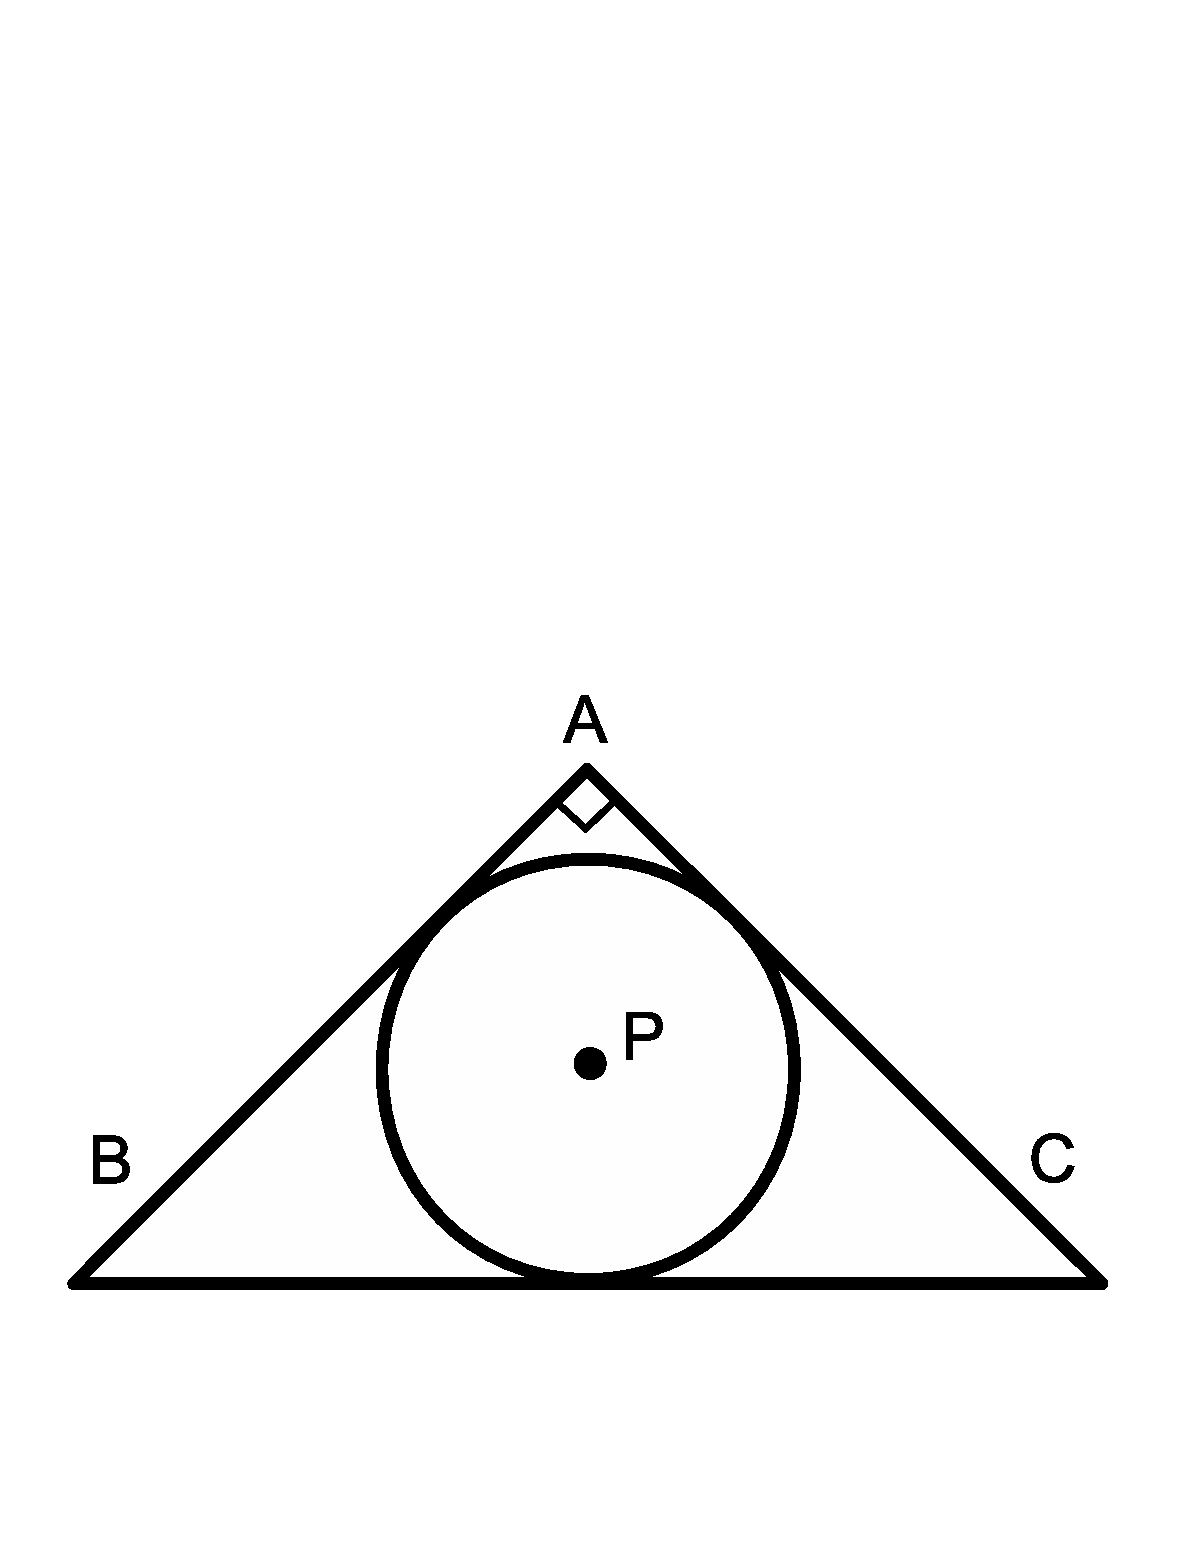
\includegraphics[width=30mm,viewport=19 116 527 413]{CCJPR74-16pic.eps}
%\end{wrapfigure}
If $x_1$ and $x_2$ are roots of the equation $x^{2}-x-1=0$, then $x_{1}+x_{2}-4x_{1}x_{2}$ equals:\\
%ChoiceA
(A) -1\\
%ChoiceB
(B) 1\\
%ChoiceC
(C) -3\\
%ChoiceD
(D) 3\\
%ChoiceE
(E) 5\\
%Ftext

%\begin{wrapfigure}{r}[0pt]{0pt}
%	\includegraphics[width=30mm,viewport=16 83 534 412]{CCJPR74-16pic2.eps}
%\end{wrapfigure}

\textbf{The correct answer is (E): 5}\\[1 ex]
Recall that the sum of the roots of the equation $ax^{2}+bx+c=0$ is $\frac{-b}{a}$, while the product of these roots is $\frac{c}{a}$. Thus, in the question, the sum of the roots, $x_{1}+x_{2}$, is $-(\frac{-1}{1})=1$ and the product of the roots $x_{1}x_{2}$, is $\frac{-1}{1}=-1$. Therefore,
\begin{equation*}
x_{1}+x_{2}-4x_{1}x_{2}=1-4\times(-1)=1+4=5.
\end{equation*}
%End
\\[5 ex]
%Begin
%Language English
%Source Cariboo College High School Mathematics competition
%Title Senior Preliminary Round 1973
%Question 17
%Subject functions
%Category concepts
%Type MC
%Choices 5
%Answer B
%Creator Victor Semenoff
%Rdifficulty 15
%Qtext

\scriptsize
Source: Cariboo College High School Mathematics Contest

\normalsize
%\begin{wrapfigure}[2]{r}[0pt]{0pt}
%	\includegraphics[width=30mm,viewport=]{CCJ78-04}
%\end{wrapfigure}
Given that $r$ is a real number, the smallest value of $3r^{2}+8$ is:\\
%ChoiceA
(A) -8\\
%ChoiceB
(B) 8\\
%ChoiceC
(C) -3\\
%ChoiceD
(D) 3\\
%ChoiceE
(E) 11\\
%Ftext

%\begin{wrapfigure}{r}[0pt]{0pt}
%	\includegraphics[width=30mm,viewport=]{CCJ78-04}
%\end{wrapfigure}

\textbf{The correct answer is (B): 8\\}\\[1 ex]
Since 8 is a constant, $3r^{2}+8$ will take on its smallest value when $3r^{2}$ takes on its smallest value.  Since $r^2$ is always positive or zero, $3r^2$ will always be positive or zero. Thus the smallest value of $3r^2$ will be zero, and the smallest value of $3r^{2}+8$ is $0+8=8$.
%End
\\[5 ex]
%Begin
%Language English
%Source Cariboo College High School Mathematics competition
%Title Senior Preliminary Round 1973
%Question 18
%Subject functions
%Category absval
%Type MC
%Choices 5
%Answer B
%Creator Victor Semenoff
%Rdifficulty 25
%Qtext

\scriptsize
Source: Cariboo College High School Mathematics Contest

\normalsize
%\begin{wrapfigure}[2]{r}[0pt]{0pt}
%	\includegraphics[width=30mm,viewport=]{CCJ78-04}
%\end{wrapfigure}
The sum of the roots of $|x|+|x-1|=3$ is:\\
%ChoiceA
(A) 0\\
%ChoiceB
(B) 1\\
%ChoiceC
(C) 2\\
%ChoiceD
(D) 3\\
%ChoiceE
(E) None of these\\
%Ftext

%\begin{wrapfigure}{r}[0pt]{0pt}
%	\includegraphics[width=30mm,viewport=]{CCJ78-04}
%\end{wrapfigure}

\textbf{The correct answer is (B): 1}\\[1 ex]
If $x\geq1$, all the terms in absolute value signs will be positive or zero, and the equation reduces to $x+x-1=3$, having the root x=2. 
If $0\leq x\leq1$, then $x$ is positive or zero, but $x-1$ is negative, and the equation reduces to 
\begin{align*}
x-(x-1)&=3\\
1&=3
\end{align*}
which, because of the inconsistency, has no roots. If $x<0$, then $x$ and $x-1$ will both be negative, and the equation will reduce to 
\begin{align*}
-x-(x-1)&=3\\
-2x+1&=3\\
\end{align*}
having the root $x=-1$.  Thus the roots of the equation are $x=2$ and $x=-1$, and the sum of the roots is $2+(-1)=1$.
%End
\\[5 ex]
%Begin
%Language English
%Source Cariboo College High School Mathematics competition
%Title Senior Preliminary Round 1973
%Question 19
%Subject geometry 
%Category angles
%Type MC
%Choices 5
%Answer B
%Creator Victor Semenoff
%Rdifficulty 23
%Qtext

\scriptsize
Source: Cariboo College High School Mathematics Contest

\normalsize
%\begin{wrapfigure}[2]{r}[0pt]{0pt}
%	\includegraphics[width=30mm,viewport=]{CCJ78-04}
%\end{wrapfigure}
If $\sin{A}=\frac{3}{5}$, then $\cos^{2}{A}+\tan^2{A}$ equals:\\
%ChoiceA
(A) $1+(\frac{4}{5})^2$\\[1 ex]
%ChoiceB
(B) $\frac{15^{2}+16^{2}}{20^{2}}$\\[1 ex]
%ChoiceC
(C) $\frac{31}{20}$\\[1 ex]
%ChoiceD
(D) $\frac{31^2}{20^2}$\\[1 ex]
%ChoiceE
(E) $(\frac{3}{14})^{2}+(\frac{4}{5})^{2}$\\
%Ftext

%\begin{wrapfigure}{r}[0pt]{0pt}
%	\includegraphics[width=30mm,viewport=]{CCJ78-04}
%\end{wrapfigure}

\textbf{The correct answer is (B): $\frac{15^{2}+16^{2}}{20^{2}}$\\[1 ex]}\\[1 ex]
If A is the angle opposite the side of length 3 in a 3-4-5 triangle, then $\sin{A}=\frac{3}{5}$. In that case, $\cos{A}=\frac{4}{5}$ and $\tan{A}=\frac{3}{4}$. Thus
\begin{equation*}
\cos^2{A}+\tan^2{A}=(\frac{4}{5})^{2}+(\frac{3}{4})^{2}=\frac{4^2\times4^2}{4^2\times5^2}+\frac{5^2\times3^2}{5^2\times4^2}=\frac{16^{2}+15^{2}}{20^2}.
\end{equation*}
%End
\\[5 ex]
%Begin
%Language English
%Source Cariboo College High School Mathematics competition
%Title Senior Preliminary Round 1973
%Question 20
%Subject functions 
%Category polynomials
%Type MC
%Choices 5
%Answer D
%Creator Victor Semenoff
%Rdifficulty 22
%Qtext

\scriptsize
Source: Cariboo College High School Mathematics Contest

\normalsize
The curve which has equation $y=ax^{2}+b$ goes through the points (1,3) and (2,8). The value of $5a+2b$ is:\\
%ChoiceA
(A) 4\\
%ChoiceB
(B) 9\\
%ChoiceC
(C) 10\\
%ChoiceD
(D) 11\\
%ChoiceE
(E) 14\\
%Ftext

\textbf{The correct answer is (D): 11}\\[1 ex]
Substituting $(x,y)=(1,3)$ into the equation for y, we obtain
\begin{align*}
3&=a\times1^{2}+b\\
a+b&=3.
\end{align*}
Substituting $(x,y)=(2,8)$ into the equation for y, we obtain
\begin{align*}
8&=a\times2^{2}+b\\
a+b&=8.
\end{align*}
Adding these two together gives
\begin{equation*}
5a+2b=3+8=11.\\
\end{equation*}
%End
\\[5 ex]
%Begin
%Language English
%Source Cariboo College High School Mathematics competition
%Title Senior Preliminary Round 1973
%Question 21
%Subject algebra
%Category modelling
%Type MC
%Choices 5
%Answer A
%Creator Victor Semenoff
%Rdifficulty 25
%Qtext

\scriptsize
Source: Cariboo College High School Mathematics Contest

\normalsize
%\begin{wrapfigure}[2]{r}[0pt]{0pt}
%	\includegraphics[width=30mm,viewport=]{CCJ78-04}
%\end{wrapfigure}
Three gallons of wine are mixed with 5 gallons of water in a barrel.  If two gallons of the mixture are drawn off and a further 1 gallon of wine added to the remainder, how many gallons of wine does 4 gallons of the new mixture contain?
%ChoiceA
(A) $1\frac{6}{7}$\\[1 ex]
%ChoiceB
(B) $2\frac{2}{7}$\\[1 ex]
%ChoiceC
(C) $2\frac{5}{7}$\\[1 ex]
%ChoiceD
(D) $3\frac{1}{4}$\\[1 ex]
%ChoiceE
(E) $3\frac{1}{2}$\\
%Ftext

%\begin{wrapfigure}{r}[0pt]{0pt}
%	\includegraphics[width=30mm,viewport=]{CCJ78-04}
%\end{wrapfigure}

\textbf{The correct answer is (A): $1\frac{6}{7}$}\\[1 ex]
The initial mixture contains 3 gallons of wine, and 5 gallons of water for a total of 8 gallons.  Since $\frac{3}{8}$ of this mixture is wine, when 2 gallons of the mixture are drawn off, $\frac{2\times3}{8}=\frac{3}{4}$ of a gallon of wine will be lost, leaving a total of $3-\frac{3}{4}=2\frac{1}{4}$ gallons of wine.  When a further 1 gallon of wine is added to this mixture, there will be a total of 7 gallons of mixture, and $3\frac{1}{4}$ gallons of wine in the mixture. Four gallons of this will contain $\frac{4}{7}$ of the total amount of wine, or
\begin{equation*}
\frac{4}{7}\times3\frac{1}{4}=\frac{4}{7}\times\frac{13}{4}=1\frac{6}{7}\textrm{ gal.}
\end{equation*}
%End
\\[5 ex]
%Begin
%Language English
%Source Cariboo College High School Mathematics competition
%Title Senior Preliminary Round 1973
%Question 22
%Subject algebra
%Category modelling
%Type MC
%Choices 5
%Answer C
%Creator Victor Semenoff
%Rdifficulty 26
%Qtext

\scriptsize
Source: Cariboo College High School Mathematics Contest

\normalsize
%\begin{wrapfigure}[2]{r}[0pt]{0pt}
%	\includegraphics[width=30mm,viewport=]{CCJ78-04}
%\end{wrapfigure}
A cougar chases a deer. The cougar takes two leaps while the deer takes three. Each leap that the cougar takes covers as much ground as two and a half of the deer's leaps. If, at the beginning of the chase, the deer was 20 of its leaps ahead of the cougar, how many leaps will the deer take before the cougar catches it?\\
%ChoiceA
(A) 60\\
%ChoiceB
(B) 40\\
%ChoiceC
(C) 30\\
%ChoiceD
(D) 17\\
%ChoiceE
(E) 10\\
%Ftext

%\begin{wrapfigure}{r}[0pt]{0pt}
%	\includegraphics[width=30mm,viewport=]{CCJ78-04}
%\end{wrapfigure}

\textbf{The correct answer is (C): 30}\\[1 ex]
Let $n$ be the number of leaps the deer takes during the chase, $d$ the distance forward that each of these leaps takes it, and $X$ the point where the cougar was at the beginning of the chase. Since the cougar takes 2 leaps for each of the deer's 3, it will take a total of $\frac{2}{3}n$ leaps during the chase. Each of the cougar's leaps moves him forward $\frac{5}{2}d$. The total distance of the deer from $X$ at the end of the chase will be $20d+nd$. The cougar's distance from X at the end of the chase will equal the number of leaps it took times the distance each of these leaps took it forward, or $\frac{2}{3}n\times \frac{5}{2}d$. The cougar and the deer are the same distance from $X$ when the deer is caught, so we set these distances equal and solve for n:
\begin{align*}
\frac{2}{3}n\times\frac{5}{2}d&=20d+nd\\
\frac{5}{3}n&=20+n\\
n&=30
\end{align*}
Thus the deer takes 30 leaps before the cougar catches it.
%End
\\[5 ex]
%Begin
%Language English
%Source Cariboo College High School Mathematics competition
%Title Senior Preliminary Round 1973
%Question 23
%Subject geometry
%Category area
%Type MC
%Choices 5
%Answer A
%Creator Victor Semenoff
%Rdifficulty 28
%Qtext

\scriptsize
Source: Cariboo College High School Mathematics Contest

\normalsize
\begin{wrapfigure}[2]{r}[0pt]{0pt}
	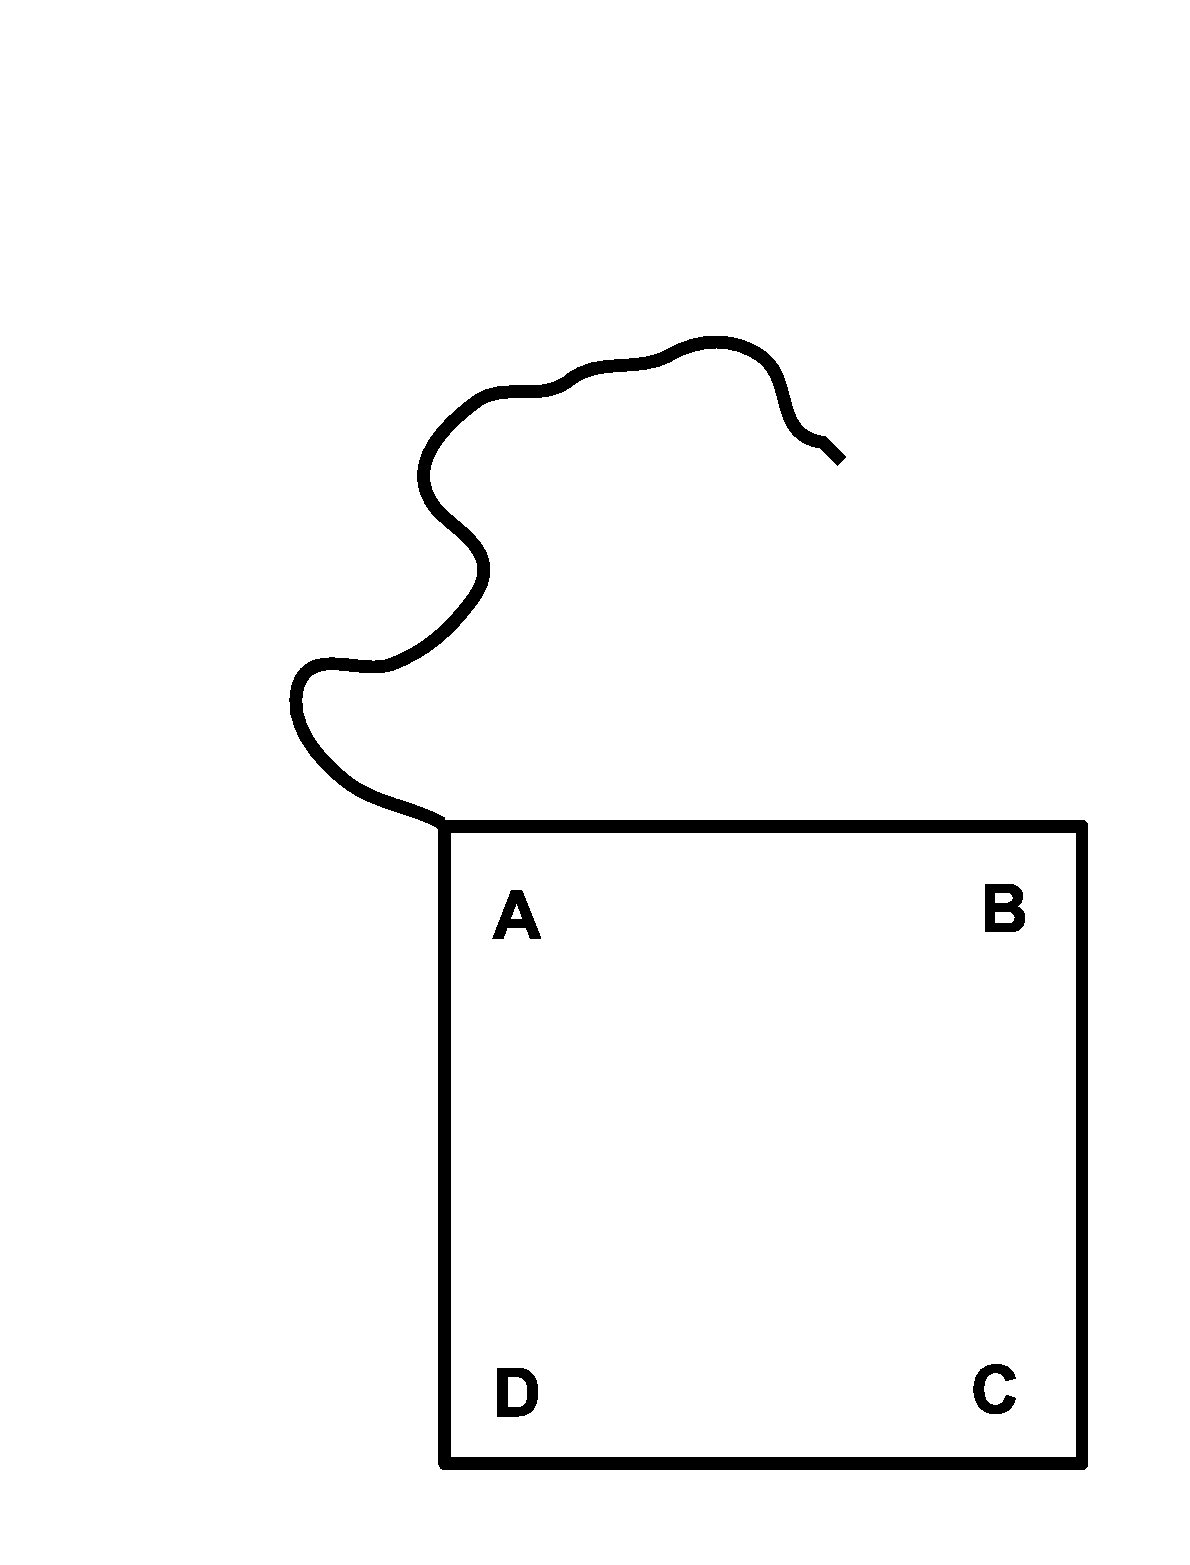
\includegraphics[width=30mm]{CCSPR73-23pic1.eps}
\end{wrapfigure}
A steer is tethered to the corner A of the square shed ABCD. If the length of the tether is 6 and the length of one side of the shed is 4, then the area that the steer can graze is:\\
%ChoiceA
(A) 29$\pi$\\
%ChoiceB
(B) $36\pi-16$\\
%ChoiceC
(C) $40\pi-16$\\
%ChoiceD
(D) 11$\pi$\\
%ChoiceE
(E) $20\pi$\\
%Ftext

\begin{wrapfigure}[8]{r}[0pt]{0pt}
	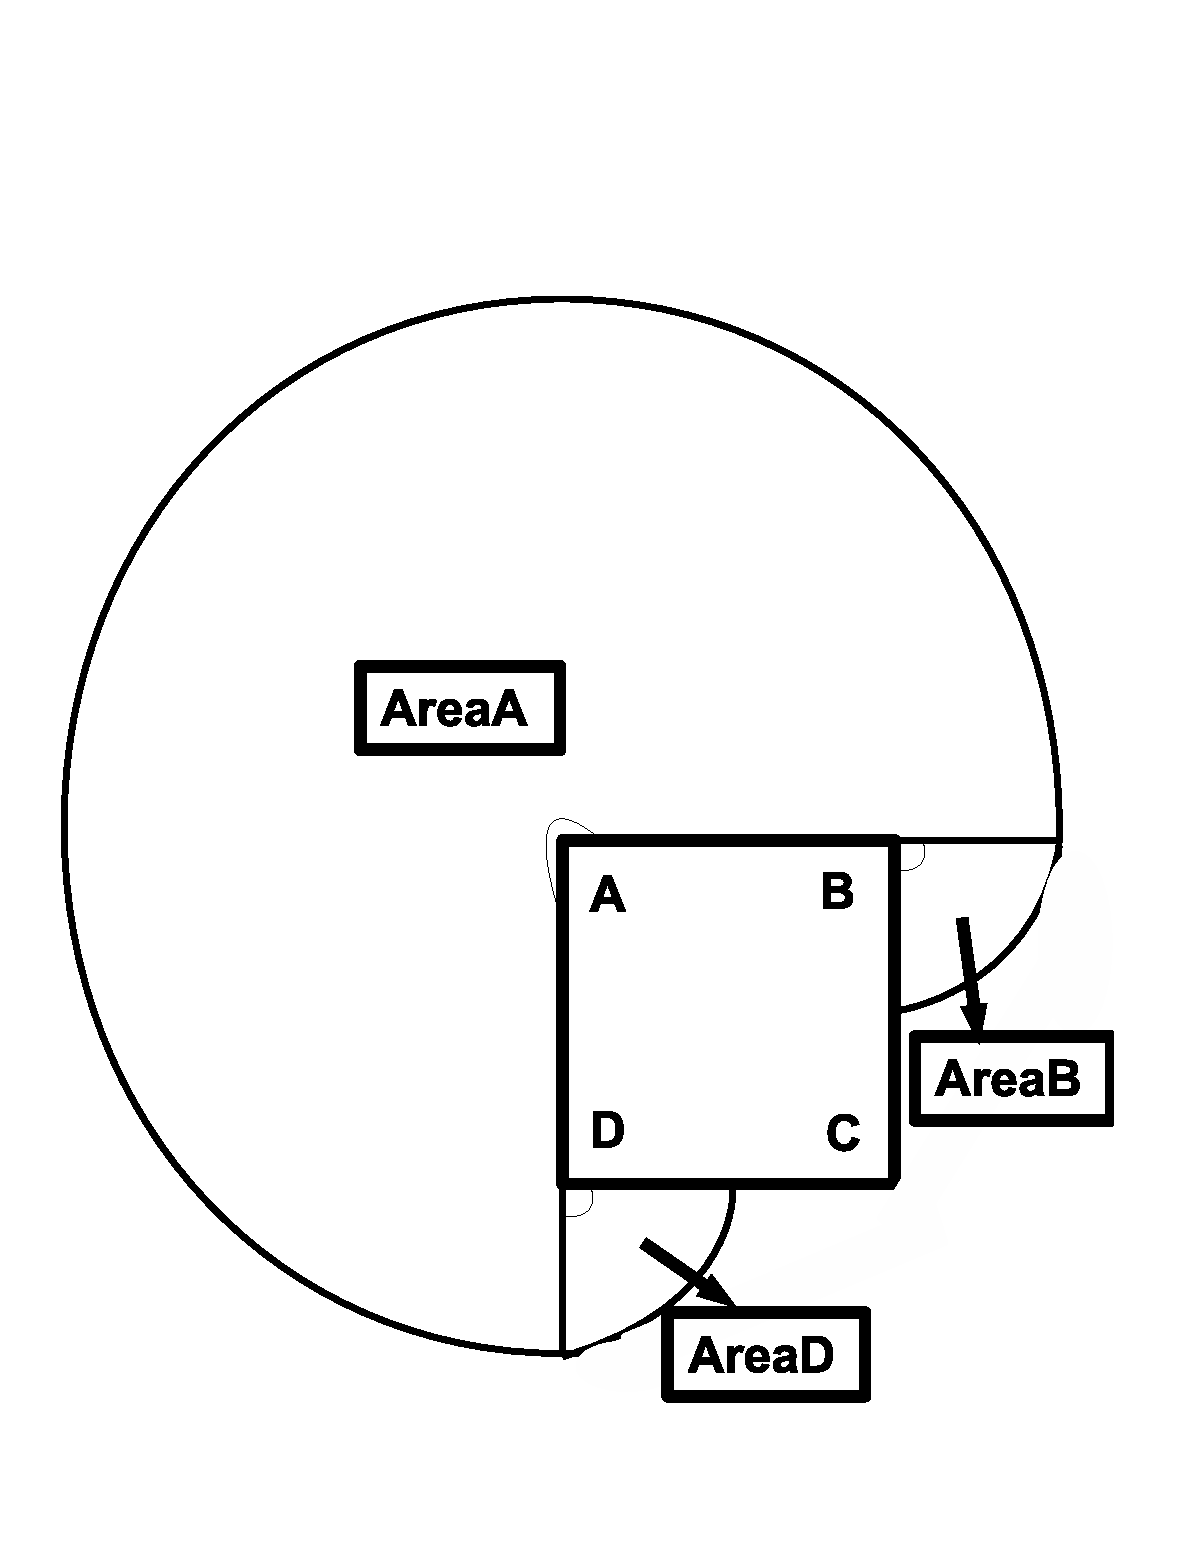
\includegraphics[width=30mm]{CCSPR73-23pic2.eps}
\end{wrapfigure}

\textbf{The correct answer is (A): 29$\pi$}\\[1 ex]
The tether has length 6, so the steer can graze in an arc of $270\,^{\circ}$ with radius 6 centered at A.  Also, there are two additional arcs centered at B and D of $90\,^{\circ}$ and radii 2.
We sum the areas bounded by the arcs and the square shed:
\begin{align*} 
\textrm{AreaA} &=\frac{270\,^{\circ}}{360\,^{\circ}}\times\pi(6)^2=27\pi\\
\textrm{AreaB} &=\frac{90\,^{\circ}}{360\,^{\circ}}\times\pi(2)^2=\pi\\
\textrm{AreaD} &=\frac{90\,^{\circ}}{360\,^{\circ}}\times\pi(2)^2=\pi\\
\end{align*}
Thus the total area is $=27\pi+\pi+\pi=29\pi$.
%End
\\[5 ex]
%Begin
%Language English
%Source Cariboo College High School Mathematics competition
%Title Senior Preliminary Round 1973
%Question 25
%Subject arithmetic
%Category integers
%Type MC
%Choices 5
%Answer E
%Creator Victor Semenoff
%Rdifficulty 29
%Qtext

\scriptsize
Source: Cariboo College High School Mathematics Contest

\normalsize
%\begin{wrapfigure}[2]{r}[0pt]{0pt}
%	\includegraphics[width=30mm,viewport=]{CCJ78-04}
%\end{wrapfigure}
Find the sum of all the integers between 1 and 1000 which are divisible by 9 or 12.\\
%ChoiceA
(A) 97,776\\
%ChoiceB
(B) 92,268\\
%ChoiceC
(C) 9,702\\
%ChoiceD
(D) 96,760\\
%ChoiceE
(E) None of these.\\
%Ftext

%\begin{wrapfigure}{r}[0pt]{0pt}
%	\includegraphics[width=30mm,viewport=]{CCJ78-04}
%\end{wrapfigure}

\textbf{The correct answer is (E): None of these.}\\[1 ex]
There are 111 multiples of 9 between 1 and 1000.  The sum of these is
\begin{equation*}
9\times1+9\times2+...+9\times111=9\times(1+2+...+111)=9\times111\times56.
\end{equation*}
There are 83 multiples of 12 between 1 and 1000.  The sum of these is
\begin{equation*}
12\times1+12\times2+...+12\times83=12\times(1+2+...+83)=12\times83\times42.
\end{equation*}
The answer we are looking for is not $9\times111\times56+12\times83\times42$ however, since we would be adding common multiples of 9 and 12 twice. We must, therefore subtract the common multiples from the sum.  The lowest common multiple of 9 and 12 is 36, and there are 27 multiples of 36 between 1 and 1000.  The sum of these is
\begin{equation*}
36\times1+36\times2+...+36\times27=36\times(1+2+...+27)=36\times\frac{27\times28}{2}=36\times27\times14.
\end{equation*}
Putting it all together we get that the sum of all the multiples of 9 and 12 between 1 and 1000 is $9\times111\times56+12\times83\times42-36\times27\times14=84,168.$
%End
\\[5 ex]
\end{document}